\documentclass{article}

% Recommended, but optional, packages for figures and better typesetting:
\usepackage{microtype}
\usepackage{graphicx}
% For some reason this is incompatible with subcaption:
%\usepackage{subfigure}
\usepackage{booktabs} % for professional tables

\usepackage[hyphens]{url}            % simple URL typesetting
\usepackage{amsmath}
\usepackage{amsfonts}       % blackboard math symbols
\usepackage{nicefrac}       % compact symbols for 1/2, etc.
\usepackage{subcaption}
\usepackage[group-separator={,}]{siunitx}
\usepackage{placeins}

% hyperref makes hyperlinks in the resulting PDF.
% If your build breaks (sometimes temporarily if a hyperlink spans a page)
% please comment out the following usepackage line and replace
% \usepackage{icml2019} with \usepackage[nohyperref]{icml2019} above.
\usepackage{hyperref}

% Attempt to make hyperref and algorithmic work together better:
\newcommand{\theHalgorithm}{\arabic{algorithm}}

% Use the following line for the initial blind version submitted for review:
% \usepackage{icml2019}

% If accepted, instead use the following line for the camera-ready submission:
\usepackage[accepted]{icml2019}

% The \icmltitle you define below is probably too long as a header.
% Therefore, a short form for the running title is supplied here:
\icmltitlerunning{Metropolis-Hastings Generative Adversarial Networks}

%\usepackage[numbers]{natbib}

\renewcommand{\vec}[1]{{\boldsymbol{\mathbf{#1}}}} % vector
\newcommand{\mat}[1]{{\ensuremath{\mathbf{#1}}}} % matrix

\newcommand{\R}{\mathbb{R}}
\newcommand{\D}{\mathcal{D}}
\newcommand{\N}{\mathcal{N}}
\newcommand{\set}[1]{\mathcal{#1}}

\newcommand{\bigO}{\mathcal{O}}
\newcommand{\ceq}{{\stackrel{c}{=}}}
\newcommand{\half}{\frac{1}{2}}
\newcommand{\T}{^\top}
\newcommand{\I}{\mathbb{I}}

\newcommand{\grad}{\nabla}
\newcommand{\sample}{\sim}
\newcommand{\given}{|}

\newcommand{\norm}{\mathcal{N}}
\newcommand{\bern}{\textrm{Bern}}

\DeclareMathOperator*{\argmin}{argmin}
\DeclareMathOperator*{\argmax}{argmax}

\newcommand{\target}{{p^\star}}
\newcommand{\prop}{q}
\newcommand{\pinit}{{p_0}}

\newcommand{\PG}{{p_G}}
\newcommand{\PD}{{p_D}}
\newcommand{\PR}{{p_{\textrm{data}}}}
\newcommand{\accept}{\alpha}

\newcommand{\setx}{\set{X}}

\newcommand{\exfactor}{1.0}
\newcommand{\pganw}{0.95in}

\begin{document}

\twocolumn[
\icmltitle{Metropolis-Hastings Generative Adversarial Networks}

% It is OKAY to include author information, even for blind
% submissions: the style file will automatically remove it for you
% unless you've provided the [accepted] option to the icml2019
% package.

% List of affiliations: The first argument should be a (short)
% identifier you will use later to specify author affiliations
% Academic affiliations should list Department, University, City, Region, Country
% Industry affiliations should list Company, City, Region, Country

% You can specify symbols, otherwise they are numbered in order.
% Ideally, you should not use this facility. Affiliations will be numbered
% in order of appearance and this is the preferred way.
\icmlsetsymbol{equal}{*}

\begin{icmlauthorlist}
\icmlauthor{Ryan Turner}{uber}
\icmlauthor{Jane Hung}{uber}
\icmlauthor{Eric Frank}{uber}
\icmlauthor{Yunus Saatci}{uber}
\icmlauthor{Jason Yosinski}{uber}
\end{icmlauthorlist}

\icmlaffiliation{uber}{Uber AI Labs}

\icmlcorrespondingauthor{Ryan Turner}{ryan.turner@uber.com}

% You may provide any keywords that you
% find helpful for describing your paper; these are used to populate
% the "keywords" metadata in the PDF but will not be shown in the document
\icmlkeywords{Metropolis Hastings, generative adversarial networks, Markov chain Monte Carlo}

\vskip 0.3in
]

% this must go after the closing bracket ] following \twocolumn[ ...

% This command actually creates the footnote in the first column
% listing the affiliations and the copyright notice.
% The command takes one argument, which is text to display at the start of the footnote.
% The \icmlEqualContribution command is standard text for equal contribution.
% Remove it (just {}) if you do not need this facility.

% Can remove this if we want more space eliminate warning
\printAffiliationsAndNotice{}  % leave blank if no need to mention equal contribution
%\printAffiliationsAndNotice{\icmlEqualContribution} % otherwise use the standard text.

\begin{abstract}
We introduce the Metropolis-Hastings generative adversarial network (MH-GAN), which combines aspects of Markov chain Monte Carlo and GANs.
The MH-GAN draws samples from the distribution implicitly defined by a GAN's discriminator-generator pair, as opposed to standard GANs which draw samples from the distribution defined only by the generator.
It uses the discriminator from GAN training to build a wrapper around the generator for improved sampling.
With a perfect discriminator, this wrapped generator samples from the true distribution on the data exactly even when the generator is imperfect.
We demonstrate the benefits of the improved generator on multiple benchmark datasets, including CIFAR-10 and CelebA, using the DCGAN, WGAN, and progressive GAN\@.
\end{abstract}

\section{Introduction}

% GANs provide implicit way to do density estimation
Traditionally, density estimation is done with a model that can compute the data likelihood.
Generative adversarial networks (GANs)~\citep{Goodfellow2014} present a radically new way to do density estimation:
They implicitly represent the density of the data via a classifier that distinguishes real from generated data.

% GAN uses D and G, but then D usually thrown away => use new method to capture knowledge captured in D, to wrap G and create a more intelligent G'
GANs iterate between updating a discriminator $D$ and a generator $G$, where $G$ generates new (synthetic) samples of data, and $D$ attempts to distinguish samples of $G$ from the real data.
In the typical setup, $D$ is thrown away at the end of training, and only $G$ is kept for generating new synthetic data points.
In this work, we propose the Metropolis-Hastings GAN (MH-GAN), a GAN that constructs a new generator $G'$ that ``wraps'' $G$ using the information contained in $D$.
This principle is illustrated in Figure~\ref{fig:intro}.\footnote{Code found at:\\ \scriptsize{\url{github.com/uber-research/metropolis-hastings-gans}}}

% Assume D is bayes optimal
The MH-GAN uses Markov chain Monte Carlo (MCMC) methods to sample from the distribution implicitly defined by the discriminator $D$ learned for the generator $G$.
This is built upon the notion that the discriminator classifies between the generator $G$ and a data distribution:
\begin{align}
  D(\vec x) = \frac{\PD(\vec x)}{\PD(\vec x) + \PG(\vec x)} \,, \label{eq:define PD}
\end{align}
where $\PG$ is the (intractable) density of samples from the generator $G$, and $\PD$ is the data density \emph{implied} by the discriminator $D$ with respect to $G$.
If GAN training reaches its global optimum, then this discriminator distribution $\PD$ is equal to the data distribution and the generator distribution ($\PD = \PR = \PG$)~\citep{Goodfellow2014}.
Furthermore, if the discriminator $D$ is optimal for a fixed imperfect generator, $G$ then the implied distribution still equals the data distribution ($\PD = \PR \neq \PG$)\@.

\begin{figure}[bhtp]
    \centering
    \begin{subfigure}[t]{2.25in}
       \centering
       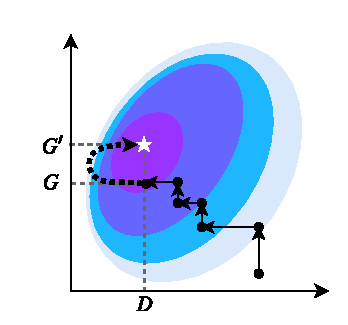
\includegraphics[scale=1.0]{figures/coord_descent.pdf}
       \caption{GAN value function}
    \end{subfigure}
    \hfill
    \begin{subfigure}[t]{3in}
       \centering
       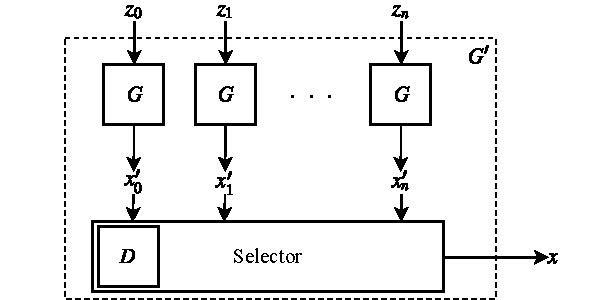
\includegraphics[scale=1.0]{figures/block_diag.pdf}
       \caption{$G'$ wraps $G$}
    \end{subfigure}
    \caption{{\small
    \textbf{(a)} We diagram how training of $D$ and $G$ in GANs performs coordinate descent on the joint minimax value function, shown in the solid black arrow.
    If GAN training produces a perfect $D$ for an imperfect $G$, the MH-GAN wraps $G$ to produce a perfect generator $G'$, as shown in the final dashed arrow.
    The generator $G$ moves vertically towards the orange region while the discriminator $D$ moves horizontally towards the purple.
    \textbf{(b)} We illustrate how the MH-GAN is essentially a selector from multiple draws of $G$.
    In the MH-GAN, the selector is built using a Metropolis-Hastings (MH) acceptance rule from the discriminator scores $D$.
    }}
    \label{fig:intro}
\end{figure}



% MCMC only needs the ratio of \PR/G and this can be found from D
We use an MCMC \emph{independence sampler}~\citep{Tierney1994} to sample from $\PD$ by taking multiple samples from $G$\@.
Amazingly, using our algorithm, one can show that given a perfect discriminator $D$ and a decent (but imperfect) generator $G$, one can obtain exact samples from the true data distribution $\PR$.
Standard MCMC implementations require (unnormalized) densities for the target $\PD$ and the proposal $\PG$, which are both unavailable for GANs.
However, the Metropolis-Hastings (MH) algorithm requires only the ratio:
\begin{align}
  \frac{\PD(\vec x)}{\PG(\vec x)} = \frac{D(\vec x)}{1 - D(\vec x)}\,, \label{eq:PD inv}
\end{align}
which we can obtain using only evaluation of $D(\vec x)$.

Sampling from an MH-GAN is more computationally expensive than a standard GAN, but the bigger and more relevant training compute cost remains unchanged.
Thus, the MH-GAN is best suited for applications where sample quality is more important than compute speed at test time.

% TODO choice between this and the "outline of this paper is as follows":
%The GAN approach to density estimation is complementary to the earlier \emph{density ratio estimation} approach~\citep{Sugiyama2012}\@.
%In density ratio estimation the generator $G$ is fixed, and the density is found by combining Bayes' rule and the learned classifier $D$.
%In GANs, the key is learning $G$ well; while in DRE, the key is learning $D$ well.
%The MH-GAN has flavors of both in that it uses both $G$ and $D$ to build $G'$.

The outline of this paper is as follows:
Section~\ref{sec:Related Work} reviews diverse areas of relevant prior work.
In Sections~\ref{sec:MCMC Methods} and~\ref{sec:GANs} we explain the necessary background on MCMC methods and GANs.
We explain our methodology of combining these two seemingly disparate areas in Section~\ref{sec:Methods} where we derive the wrapped generator $G'$.
Results on real data (CIFAR-10 and CelebA) and extending common GAN models (DCGAN, WGAN, and progressive GAN) are shown in Section~\ref{sec:Results}.
Section~\ref{sec:conclusions} discusses implications and conclusions.

\section{Related Work}
\label{sec:Related Work}

% Need to be clear on diff with NICE-MCMC
A few other works combine GANs and MCMC in some way.
\citet{Song2017} use a GAN-like procedure to train a RealNVP~\citep{Dinh2016} MCMC proposal for sampling an externally provided target \smash{$\target$}.
Whereas \citet{Song2017} use GANs to accelerate MCMC, we use MCMC to enhance the samples from a GAN\@.
Similar to \citet{Song2017}, \citet{Kempinska2017} improve proposals in particle filters rather than MCMC\@.
\citet{Song2017} was recently generalized by~\citet{Neklyudov2018}.

\subsection{Discriminator Rejection Sampling}
A concurrent work with similar aims from~\citet{Azadi2018} proposes discriminator rejection sampling (DRS) for GANs, which performs rejection sampling on the outputs of $G$ by using the probabilities given by $D$.
While conceptually appealing at first, DRS suffers from two major shortcomings in practice.
First, it is necessary to find an upper-bound on $D$ over all possible samples in order to obtain a valid proposal distribution for rejection sampling.
Because this is not possible, one must instead rely on estimating this bound by drawing many pilot samples.
Secondly, even if one were to find a good bound, the acceptance rate would become very low due to the high-dimensionality of the sampling space.
This leads~\citet{Azadi2018} to use an extra $\gamma$ heuristic to shift the logit $D$ scores, making the model sample from a distribution different from $\PR$ even when $D$ is perfect.
We use MCMC instead, which was invented precisely as a replacement for rejection sampling in higher dimensions.
We further improve the robustness of MCMC via use of a \emph{calibrator} on the discriminator to get more accurate probabilities for computing acceptance.  % probabilities

\section{Background and Notation}
\label{sec:Background}

In this section, we briefly review the notation and equations with MCMC and GANs.

\subsection{MCMC Methods}
\label{sec:MCMC Methods}

MCMC methods attempt to draw a chain of samples $\vec x_{1:K} \in \setx^K$ that marginally come from a target distribution $\target$.
We refer to the initial distribution as $\pinit$ and the proposal for the independence sampler as $\vec x' \sample \prop(\vec x' \given \vec x_k)=\prop(\vec x')$.
The proposal $\vec x' \in \setx$ is accepted with probability
\begin{align}
  \accept(\vec x', \vec x_k) = \min\left(1, \frac{\target(\vec x')\prop(\vec x_k)}{\target(\vec x_k)\prop(\vec x')}\right) \in [0,1]\,. \label{eq:alpha def}
\end{align}
If $\vec x'$ is accepted, $\vec x_{k+1} = \vec x'$, otherwise $\vec x_{k+1} = \vec x_k$.
Note that when estimating the distribution $\target$, one must include the duplicates that are a result of rejections in $\vec x'$.

\paragraph{Independent samples}
Many evaluation metrics assume perfectly iid samples.
Although MCMC methods are typically used to produce correlated samples, we can produce iid samples by using one chain per sample:
Each chain samples $\vec x_0 \sample \pinit$ and then does $K$ MH iterations to get $\vec x_K$ as the output of the chain, which is the output of $G'$.
Using multiple chains is also better for GPU parallelization.

\paragraph{Detailed balance}
The detailed balance condition implies that if $\vec x_k \sample \target$ exactly then $\vec x_{k+1} \sample \target$ exactly as well.
Even if $\vec x_k$ is not exactly distributed according to $\target$, the Kullback-Leibler (KL) divergence between the implied density it is drawn from and $\target$ always decreases as $k$ increases~\citep{Murray2008}.
We use detailed balance to motivate our approach to MH-GAN initialization.

%The curious reader may wonder why we do not simply stop the chain after the first accept.
%In general, allowing chain length $K$ to be conditioned in any way on the state of the chain (including which samples were accepted or rejected) has the potential to introduce bias to the samples~\citep{Cowles1999}.

\subsection{GANs}
\label{sec:GANs}

GANs implicitly model the data $\vec x$ via a synthetic data generator \smash{$G \in \R^{d} \rightarrow \setx$}:
\begin{align}
  \vec x = G(\vec z)\,, \quad \vec z \sample \norm(\vec 0, \vec I_{d})\,.
\end{align}
This implies a (intractable) distribution on the data $\vec x \sample \PG$.
We refer to the unknown true distribution on the data $\vec x$ as $\PR$.
The discriminator $D \in \setx \rightarrow [0,1]$ is a soft classifier predicting if a data point is real as opposed to being sampled from $\PG$\@.

If $D$ converges optimally for a fixed $G$, then \smash{$D = \PR/(\PR + \PG)$}, and if both $D$ and $G$ converge then $\PG = \PR$~\citep{Goodfellow2014}.
GAN training forms a game between $D$ and $G$.
In practice $D$ is often better at estimating the density ratio than G is at generating high-fidelity samples~\citep{Shibuya2017}.
This motivates wrapping an imperfect $G$ to obtain an improved $G'$ by using the density ratio information contained in $D$.

\begin{figure}[htbp]
    \centering
    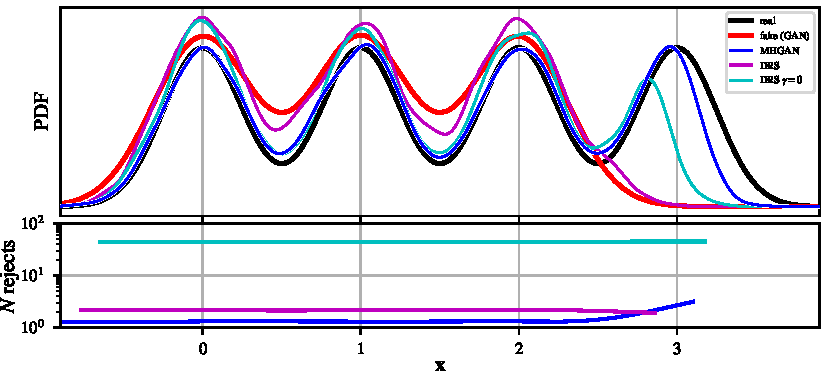
\includegraphics[scale=1.0]{figures/univariate_example.pdf}
    \caption{{\small
    Illustration comparing the MH-GAN setup with the formulation of DRS on a univariate example.
    This figures uses a $\PR$ of four Gaussian mixtures while $\PG$ is missing one of the mixtures.
    The top row shows the resulting density of samples, while the bottom row shows the typical number of rejects before accepting a sample at that $\vec x$ value.
    The MH-GAN recovers the true density except in the far right tail where there is an exponentially small chance of getting a sample from the proposal $\PG$.
    DRS with $\gamma=0$ shift should also be able to recover the density exactly, but it has an even larger error in the right tail.
    These errors arise because we must approximate the max $D$ score and use only \num{10000} pilot samples to do so, as in \citet{Azadi2018}.
    Additionally, due to the large maximum $D$, it needs a large number of draws before a single accept.
    DRS with $\gamma$ shift is much more sample efficient, but completely misses the right mode as the setup invalidates the rejection sampling equations.
    The MH-GAN is more adaptive in that it quickly accepts samples for the areas $\PG$ models well; more MCMC rejections occur before accepting a sample in the right poorly modeled mode.
    However, in all cases the MH-GAN is more efficient than DRS without $\gamma$ shift.
    Presumably, this effect only becomes greater in higher dimensions.
    }}
    \label{fig:univariate_example}
\end{figure}



\section{Methods}
\label{sec:Methods}

% Derive basic trick for MCMC using D
In this section we show how to sample from the distribution $\PD$ implied by the discriminator $D$.
We apply~\eqref{eq:PD inv} and~\eqref{eq:alpha def} for a target of $\target=\PD$ and proposal $\prop=\PG$:
\begin{align}
  \frac{\PD}{\PG} &= \frac{1}{D^{-1} - 1} \\
  \implies
  \accept(\vec x', \vec x_k) &= \min\left(1, \frac{D(\vec x_k)^{-1} - 1}{D(\vec x')^{-1} - 1}\right)\,. \label{eq:alpha from D}
\end{align}
The ratio $\PD/\PG$ is computed entirely from the discriminator scores $D$.
If $D$ is perfect, $\PD = \PR$, so the sampler will marginally sample from $\PR$.
The use of~\eqref{eq:alpha from D} is further illustrated in Algorithm~\ref{alg:mhgan}.

A toy one-dimensional example with just such a perfect discriminator is shown in Figure~\ref{fig:univariate_example}.
In this example the MH-GAN is able to correctly reconstruct a missing mode in the generating distribution from the tail of a faulty generator.

\paragraph{Calibration}
The probabilities for $D$ must not merely provide a good AUC score, but must also be well \emph{calibrated}.
In other words, if one were to warp the probabilities of the perfect discriminator in~\eqref{eq:define PD} it may still suffice for standard GAN training, but it will not work in the MCMC procedure defined in~\eqref{eq:alpha from D}, as it will result in erroneous density ratios.

We can demonstrate the miscalibration of $D$ using the statistic of~\citet{Dawid1997} on held out samples \smash{$\vec x_{1:N}$} and real/fake labels \smash{$y_{1:N} \in \{0,1\}^N$}.
If $D$ is well calibrated, i.e., $y$ is indistinguishable from a \smash{$y \sample \bern(D(\vec x))$}, then
\begin{align}
  Z = \frac{\sum_{i=1}^N y_i - D(\vec x_i)}{\sqrt{\sum_{i=1}^N D(\vec x_i) (1 - D(\vec x_i))}} \!\!\implies\!\! Z \sample \norm(0,1)\,. \label{eq:calib score}
\end{align}
That is, we expect the $Z$ diagnostic to be a Gaussian in large $N$ for any well-calibrated classifier.
This means that for large values of $Z$, such as when $|Z| > 2$, we reject the hypothesis that $D$ is well-calibrated.
%Note this statistic is \emph{not} used for recalibration, but rather to demonstrate that GAN discriminators are typically poorly calibrated.

\paragraph{Correcting Calibration}
While~\eqref{eq:calib score} may tell us a classifier is poorly calibrated, we also need to be able to fix it.
Furthermore, some GANs (like WGAN) require calibration because their discriminator only outputs a score and not a probability.
To correct an uncalibrated classifier, denoted $\tilde{D} \in \setx \rightarrow \R$, we use a \emph{held out} calibration set (e.g., 10\% of the training data) and either logistic, isotonic, or beta~\citep{Kull2017} regression to warp the output of $\tilde{D}$.
The held out calibration set contains an equal number of positive and negative examples, which in the case of GANs is an even mix of real samples and fake samples from $G$.
After $\tilde{D}$ is learned, we train a probabilistic classifier $C \in \R \rightarrow [0,1]$ to map $\tilde{D}(\vec x_i)$ to $y_i$ using the calibration set.
The calibrated classifier is built via $D(\vec x_i) = C(\tilde{D}(\vec x_i))$.
%When the calibration set is large nonparametric methods such as isotonic regression usually perform the best while beta calibration tends to be better for small calibration sets.

\paragraph{Initialization}
We also avoid the burn-in issues that usually plague MCMC methods.
Recall that via the detailed balance property~\citep[Ch.~1]{Gilks1996}, if the marginal distribution of a Markov chain state $\vec x \in \setx$ at time step $k$ matches the target $\PD$ (\smash{$\vec x_k \sample \PD$}), then the marginal at time step $k+1$ will also follow $\PD$ (\smash{$\vec x_{k+1} \sample \PD$})\@.
In most MCMC applications it is not possible to get an initial sample from the target distribution (\smash{$\vec x_0 \sample \PD$})\@.

However, for MH-GAN, we have access to real data from the target distribution.
By initializing the chain at a sample of real data (the correct distribution), we apply the detailed balance property and avoid burn-in.
If no generated sample is accepted by the end of the chain, we restart sampling from a synthetic sample to ensure the initial real sample is never output.
To make restarts rare, we set $K$ large (often 640)\@.

Using a restart after an MCMC chain of only rejects has a theoretical potential for bias.
However, MCMC in practice often uses chain diagnostics as a stopping criterion, which suffers the same bias potential~\citep{Cowles1999}.
Alternatively, we could never restart and always report the state after $K$ samples, which will occasionally include the initial real sample.
This might be a better approach in certain statistical problems, where we care more about eliminating any potential source of bias, than in image generation.

% Note how requirement not that strong with calibration and manifold
\paragraph{Perfect Discriminator}
The assumption of a perfect $D$ may be weakened for two reasons:
(A)~Because we recalibrate the discriminator, the actual probabilities can be incorrect as long as the decision boundary between real and fake is correct.
(B)~Because the discriminator is only ever evaluated at samples from $G$ or the initial real sample $\vec x_0$, $D$ only needs to be accurate on the manifold of samples from the generator $\PG$ and the real data $\PR$.

\begin{figure}[tbp]
    \centering
    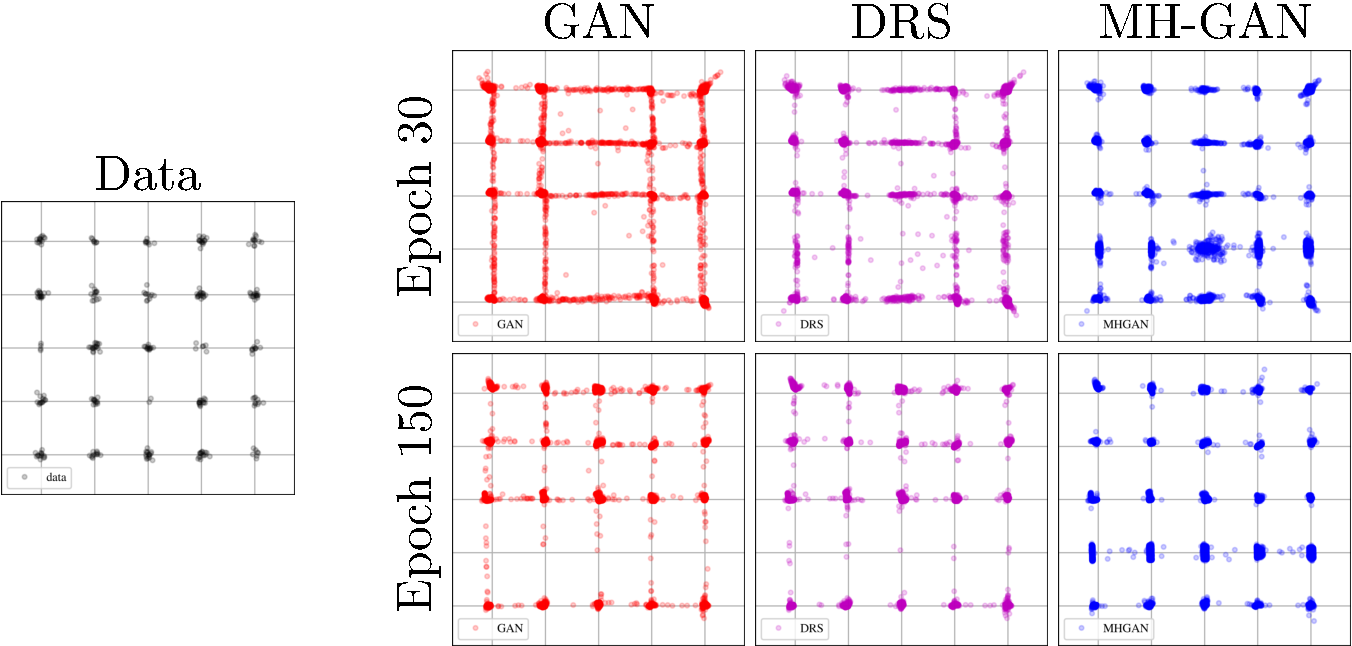
\includegraphics[width=1.0\linewidth]{figures/mog_unified.pdf}
    \caption{{\small
    Data in the 25 Gaussians example (upper-left)\@.
    The other GAN setups are shown in the other figures.
    The MH-GAN corrects areas of mis-assigned mass in the original GAN\@.
    DRS appears visually closer to the original GAN than the data, whereas the MH-GAN appears closer to the actual data.
    We show the state of the generators at epoch 30 (when MH-GAN begins showing large gains) on the left and epoch 150 (the final epoch) on the right.
    }}
    \label{fig:mog_example}
\end{figure}



\begin{algorithm}[tb]
   \caption{MH-GAN}
   \label{alg:mhgan}
\begin{algorithmic}
   \STATE {\bfseries Input:} generator $G$, calibrated disc.~$D$, real samples
   \STATE Assign random real sample $\vec x_0$ to $\vec x$
   \FOR{$k=1$ {\bfseries to} $K$}
   \STATE Draw $\vec x'$ from $G$
   \STATE Draw $U$ from $\textrm{Uniform}(0,1)$
   \IF{\smash{$U \leq (D(\vec x)^{-1} - 1) / (D(\vec x')^{-1} - 1)$}}
   \STATE $\vec x \leftarrow \vec x'$
   \ENDIF
   \ENDFOR
   \STATE If $\vec x$ is still real sample $\vec x_0$ restart with draw from $G$ as $\vec x_0$
   \STATE {\bfseries Output:} sample $\vec x$ from $G'$
\end{algorithmic}
\end{algorithm}



\section{Results}
\label{sec:Results}

We first show an illustrative synthetic mixture model example followed by real data with images.

\subsection{Mixture of 25 Gaussians}

We consider the $5 \times 5$ grid of two-dimensional Gaussians used in~\citet{Azadi2018}, which has become a popular toy example in the GAN literature~\citep{Dumoulin2016}.
The means are arranged on the grid $\mu \in \{{-2},{-1},0,1,2\}$ and use a standard deviation of $\sigma = 0.05$.

\paragraph{Experimental setup}
Following~\citet{Azadi2018}, we use four fully connected layers with ReLU activations for both the generator and discriminator.
The final output layer of the discriminator is a sigmoid, and no nonlinearity is applied to the final generator layer.
All hidden layers have size 100, with a latent \smash{$\vec z \in \R^2$}.
We used \num{64000} standardized training points and generated \num{10000} points in test.

\paragraph{Visual results}
In Figure~\ref{fig:mog_example}, we show the original data along with samples generated by the GAN\@.
We also show samples enhanced via the MH-GAN (with calibration) and with DRS\@.
The standard GAN creates spurious links along the grid lines between modes and misses some modes along the bottom row.
DRS is able to reduce some of the spurious links but not fill in the missing modes.
The MH-GAN further reduces the spurious links and recovers these under-estimated modes.

\paragraph{Quantitative results}
These results are made more quantitative in Figure~\ref{fig:mog_metrics}, where we follow some of the metrics for the example from~\citet{Azadi2018}.
We consider the standard deviations within each mode in Figure~\ref{fig:std} and the rate of ``high quality'' samples in Figure~\ref{fig:hqr}.
A sample is assigned to a mode if its $L_2$ distance is within four standard deviations ($\leq 4 \sigma = 0.2$) of its mean.
Samples within four standard deviations of any mixture component are considered ``high quality''.
The within standard deviation plot~(Figure~\ref{fig:std}) shows a slight improvement for MH-GAN, and the high quality sample rate~(Figure~\ref{fig:hqr}) approaches 100\% faster for the MH-GAN than the GAN or DRS\@.

To test the spread of the distribution, we inspect the categorical distribution of the closest mode.
Far away (non-high quality) samples are assigned to a 26th unassigned category.
This categorical distribution should be uniform over the 25 real modes for a perfect generator.
To assess generator quality, we look at the Jensen-Shannon divergence (JSD) between the sample mode distribution and a uniform distribution.
This is a much more stringent test of appropriate spread of probability mass than checking if a single sample is produced near a mode (as in~\citet{Azadi2018})\@.

\begin{figure}[htbp]
    \centering
    \begin{subfigure}[b]{0.32\textwidth}
       \centering
       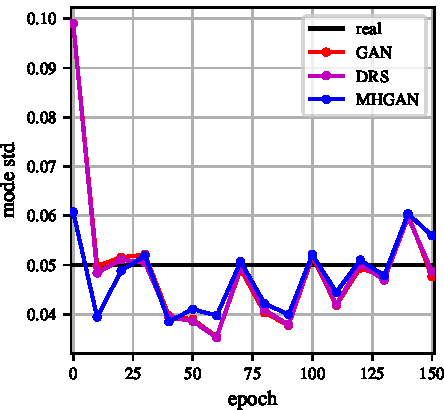
\includegraphics[width=1.8in]{figures/std.pdf}
       \caption{mode std.~dev.}
       \label{fig:std}
    \end{subfigure}
    \begin{subfigure}[b]{0.32\textwidth}
       \centering
       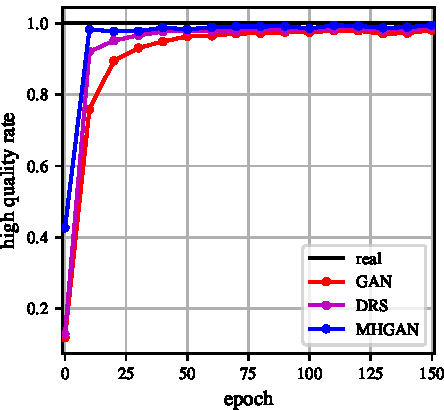
\includegraphics[width=1.8in]{figures/hqr.pdf}
       \caption{high quality rate}
       \label{fig:hqr}
    \end{subfigure}
    \begin{subfigure}[b]{0.32\textwidth}
       \centering
       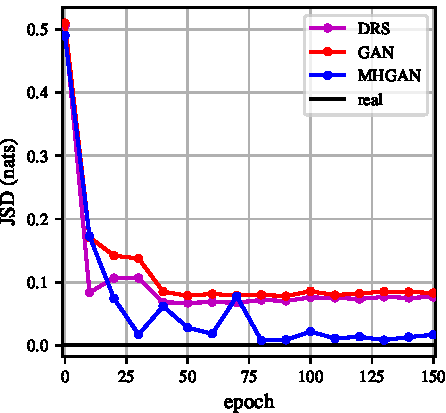
\includegraphics[width=1.8in]{figures/jsd.pdf}
       \caption{Jensen-Shannon divergence}
       \label{fig:jsd}
    \end{subfigure}
    \caption{{\small
    Results of the MH-GAN experiments on the mixture of 25 Gaussians example.
    On the left, we show the standard deviation of samples within a single mode.
    The black line represents the scores the true distribution.
    In the center, we show the high quality rate (samples near a real mode) across different GAN setups.
    On the right, we show the Jensen-Shannon divergence (JSD) between the distribution on the nearest mode vs a uniform, which is the generating distribution on mixture components.
    The MH-GAN shows, on average, a $5 \times$ improvement in JSD over DRS\@.
    We considered adding error bars to these plots via a bootstrap analysis, but the error bars are too small to be visible.
    }}
    \label{fig:mog_metrics}
\end{figure}


\begin{figure}[htbp]
    \centering
    \begin{subfigure}[b]{0.32\textwidth}
       \centering
       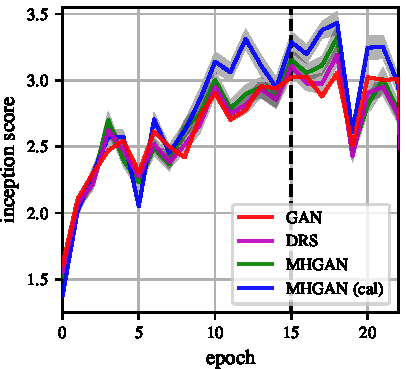
\includegraphics[width=1.8in]{figures/per_epoch.pdf}
       \caption{performance by epoch}
       \label{fig:incep_by_epoch}
    \end{subfigure}
    \begin{subfigure}[b]{0.32\textwidth}
       \centering
       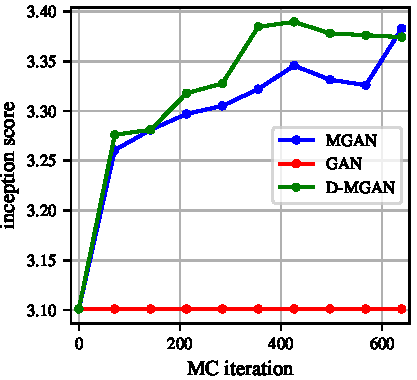
\includegraphics[width=1.8in]{figures/plot_per_mh.pdf}
       \caption{performance by MCMC iteration}
       \label{fig:incep_by_iter}
    \end{subfigure}
    \begin{subfigure}[b]{0.32\textwidth}
       \centering
       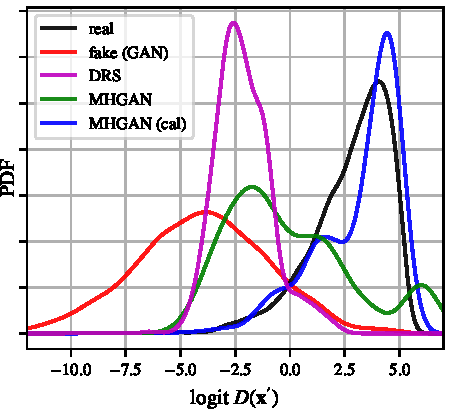
\includegraphics[width=1.8in]{figures/score_dist_bta.pdf}
       \caption{epoch 13 scores}
       \label{fig:score_dist_overlap}
    \end{subfigure}
    \caption{{\small
    Results of the MH-GAN experiments on CIFAR-10 using the DCGAN\@.
    On the left, we show the inception score by training epoch of the DCGAN at $K=640$.
    MH-GAN denotes using the raw discriminator scores and ``MH-GAN (cal)'' for the calibrated scores.
    The error bars on MH-GAN performance (in gray) are computed using a t-test on the variation per batch across 80 splits of the inception score.
    In the center we show the inception score vs.~MCMC iteration $k$ for the GAN at epoch 15.
    On the right, we show the scores at epoch 13 where there is some overlap between the scores of fake and real images.
    When there is overlap, the MH-GAN corrects the $\PG$ distribution to have scores looking similar to the real data.
    DRS fails to fully shift the distribution because 1)~it does not use calibration and 2)~its ``$\gamma$ shift'' setup violates the validity of rejection sampling.
    }}
    \label{fig:inception}
\end{figure}



In Figure~\ref{fig:jsd}, we see that the MH-GAN improves the JSD over DRS by $5 \times$ on average, meaning it achieves a much more balanced spread across modes.
DRS fails to make gains after epoch 30.
Using the principled approach of the MH-GAN along with calibrated probabilities ensures a correct spread of probability mass.

\subsection{Real Data}

For real data experiments we considered the CelebA~\citep{Liu2015} and CIFAR-10~\citep{Torralba2008} data sets modeled using the DCGAN~\citep{Radford2015} and WGAN~\citep{Arjovsky2017, Gulrajani2017}.
To evaluate the generator $G'$, we plot Inception scores~\citep{Salimans2016} per epoch in Figure~\ref{fig:incep_by_epoch} after $K=640$ MCMC iterations.
%The actual performance boost realized by MH-GAN oscillates from one epoch to the next, perhaps due to fluctuations in the density ratio estimation performance per epoch.
%Accordingly the statistical significance of the boost from $G$ to $G'$ with calibration varies from no significant change to boost with \smash{$p < 10^{-4}$}.
Figure~\ref{fig:incep_by_iter} shows Inception score per MCMC iteration:
most gains are made in the first $k=100$ iterations, but gains continue to $k=400$.
This shows that the MH-GAN allows a tunable trade-off between sample quality and computation cost.

\begin{figure*}
    \centering
    \begin{subfigure}[b]{0.49\textwidth}
       \centering
       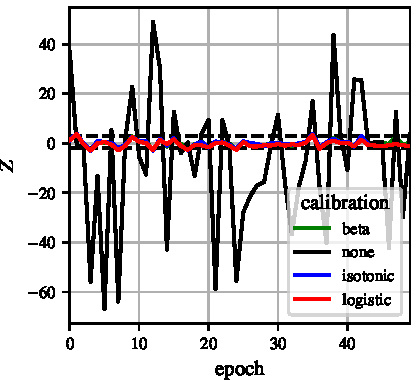
\includegraphics[scale=0.95]{figures/disc_calib_cifar.pdf}
       \caption{CIFAR-10}
       \label{fig:calibration cifar}
    \end{subfigure}
    \begin{subfigure}[b]{0.49\textwidth}
       \centering
       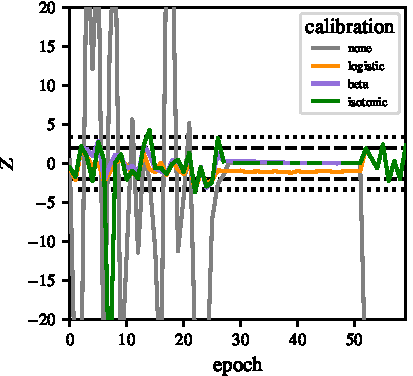
\includegraphics[scale=0.95]{figures/disc_calib_celeba.pdf}
       \caption{CelebA}
       \label{fig:calibration CelebA}
    \end{subfigure}
    \caption{{\small
    We show the calibration statistic $Z$~\eqref{eq:calib score} for the discriminator on held out data for the DCGAN\@.
    The results for CIFAR-10 are shown on the right, and CelebA on the left.
    The raw discriminator is clearly miscalibrated being far outside the region expected by chance (dashed black), and after multiple comparison correction (dotted black)\@.
    All the calibration methods give roughly equivalent results.
    CelebA has a period of training instability during epochs 30--50 which gives trivially calibrated classifiers.
    }}
    \label{fig:calibration}
\end{figure*}

\begin{table}[htbp]
\begin{center}
  \caption{{\small
    Results showing Inception score improvements from MH-GAN on DCGAN and WGAN at epoch 60.
    Like Figure~\ref{fig:incep_by_epoch}, the error bars and p-values are computed using a paired t-test across Inception score batches.
    All results except for DCGAN on celebA are significant at \smash{$p < 10^{-4}$}.
    WGAN does not learn a typical GAN discriminator that outputs a probability, so calibration is actually required in this case.
    }}
    \label{tbl:inception}
{\scriptsize
\begin{tabular}{|l|l|r|l|r||l|r|l|r|}
\toprule
~                 & \multicolumn{4}{c||}{DCGAN}                               & \multicolumn{4}{c|}{WGAN} \\
\toprule
~            & {CIFAR-10}                &      p   & CelebA                  &      p   & CIFAR-10                 &       p  & CelebA                 &       p  \\
\midrule
%\hline \\
GAN          &        2.8789             &       -- &      2.3317             &       -- &       3.0734             &       -- &     2.7876             &       -- \\
DRS          &        2.977(77)          &   0.0131 &      2.511(50)          &  <0.0001 &               ~          &        ~ &             ~          &        ~ \\
DRS (cal)    &        3.073(80)          &  <0.0001 &      2.869(67)          &  <0.0001 &       3.137(64)          &   0.0497 &     2.861(66)          &   0.0277 \\
MH-GAN       &        3.113(69)          &  <0.0001 &      2.682(50)          &  <0.0001 &               ~          &        ~ &             ~          &        ~ \\
MH-GAN (cal) &        \textbf{3.379}(66) &  <0.0001 &      \textbf{3.106}(64) &  <0.0001 &       \textbf{3.305}(83) &  <0.0001 &     \textbf{2.889}(89) &   0.0266 \\
\bottomrule
\end{tabular}
}
\end{center}
\end{table}



In Table~\ref{tbl:inception}, we summarize performance (Inception score) across all experiments, running MCMC with $K=640$ iterations in all cases.
Behavior is qualitatively similar to that in Figure~\ref{fig:incep_by_epoch}.
While DRS improves on a direct GAN, MH-GAN improves Inception score more in every case.
Calibration helps in every case;
and we found a slight advantage for isotonic regression over other calibration methods.
Results are computed at epoch 60, and as in Figure~\ref{fig:incep_by_epoch}, error bars and p-values are computed using a paired t-test across Inception score batches.
All results are significantly better than the baseline GAN at \smash{$p < 0.05$}.

\paragraph{Score distribution}
In Figure~\ref{fig:score_dist_overlap}, we show what $G'$ does to the distribution on discriminator scores.
MCMC shifts the distribution of the fakes to match the distribution on true images.
We also observed that the MH acceptance rate is primarily determined by the overlap of the distributions on $D$ scores between real and fake samples.
%In other words, how good the generator $G$ is at tricking the discriminator $D$.
If the AUC of $D$ is less than 0.90 we see acceptance rates over 20\%; but when the AUC of $D$ is 0.95, accept rates drop to 10\%.

\paragraph{Calibration results}
Figure~\ref{fig:calibration} shows the results per epoch for both CIFAR-10 and CelebA\@.
It shows that the raw discriminator is highly miscalibrated, but can be fixed with any of the standard calibration methods.
The $Z$ statistic for the raw discriminator $D$ (DCGAN on CIFAR-10) varies from $-77.57$ to $48.98$ in the first 60 epochs; even after Bonferroni correction at $N \!\!=\!\! 60$, we expect $|Z| < 3.35$ with 95\% confidence for a calibrated classifier.
The calibrated discriminator varies from $-2.91$ to $3.60$, which shows it is almost perfectly calibrated.
Accordingly, it is unsurprising that the calibrated discriminator significantly boosts performance in the MH-GAN\@.

\paragraph{Visual results}
We also show example images from the CIFAR-10 and CelebA setups in the supplementary material.
The selectors (such as MH-GAN) result in a wider spread of probability mass across background colors.
For CIFAR-10, it enhances modes with animal-like outlines and vehicles.

\subsection{Progressive GAN}

To further illustrate the power of the MH-GAN approach we consider the progressive GAN (PGAN)~\citep{Karras2017}, which recently produced shockingly realistic images.
We applied the MH-GAN to a PGAN using the same setup as with DCGAN, using $K=800$.
We used the pre-trained network of~\citet{Karras2017} on CelebA-HQ (1024$\times$1024)\@.
Large batches of samples are in the supplementary material.

In Table~\ref{tbl:pgan}, we use the progressive GAN as our base GAN and generate random samples from the base, as well as from the addition of DRS and MH-GAN selectors.
The different selectors (DRS and MH-GAN) are run on the same batches of images,
so the same images may appear for both generators.

Although, the progressive GAN sometimes produces near photo realistic images, it also produces many flawed nightmare like images.
Both DRS and MH-GAN show an ability to select just the realistic images.
The MH-GAN samples are nearly perfect, while DRS still has many flawed samples.

\section{Conclusions}
\label{sec:conclusions}

We have shown how to incorporate the knowledge in the discriminator $D$ into an improved generator $G'$.
Our method is based on the premise that $D$ is better at density ratio estimation than $G$ is at sampling data, which may be a harder task.
The principled MCMC setup selects among samples from $G$ to correct biases in $G$.
This is the only method in the literature which has the property that given a perfect $D$ one can recover $G$ such that $\PG = \PR$.

We have shown the raw discriminators in GANs and DRS are poorly calibrated.
To our knowledge, this is the first work to evaluate the discriminator in this way and to rigorously show the poor calibration of the discriminator.
The MH-GAN has great potential for extension. \todo{how?}

\fboxsep=1.5pt  % padding thickness
\newcommand{\unreal}[1]{\fcolorbox{white}{red}{#1}}

\begin{table*}[htbp]
\vspace{-3mm}  % alignment looks a little better
\begin{center}
  \caption{{\small
    % Random samples using a pre-trained PGAN as the base GAN\@.
    % Since the PGAN does not output a probability, we must calibrate the scores by isotonic regression.
    We show 16 \emph{random samples} from the PGAN, calibrated (improved) DRS, and MH-GAN, from the same sequence of $G$ samples.
    There are 5 cases where the PGAN produces bad warpings (red) while the MH-GAN does not, and 0 cases where the MH-GAN does and the PGAN does not;
    for DRS, there are 7 where only DRS is warped, and 1 where only MH-GAN is warped.
    Even with 16 samples, the MH-GAN is better under a one-sided pairwise trinomial test~\citep{Coakley1996} at $p=0.017$ vs DRS and $p=0.013$ vs PGAN\@.
    }}
  \label{tbl:pgan}
\setlength\tabcolsep{1pt} % default value: 6pt
\begin{tabular}{cc|cc|cc}
\multicolumn{2}{c|}{PGAN} & \multicolumn{2}{c|}{DRS (cal)} & \multicolumn{2}{c}{MH-GAN (cal)} \\
\toprule
\unreal{
\includegraphics[width=\pganw]{figures/pgan/48_base_iso_base.jpg}} &
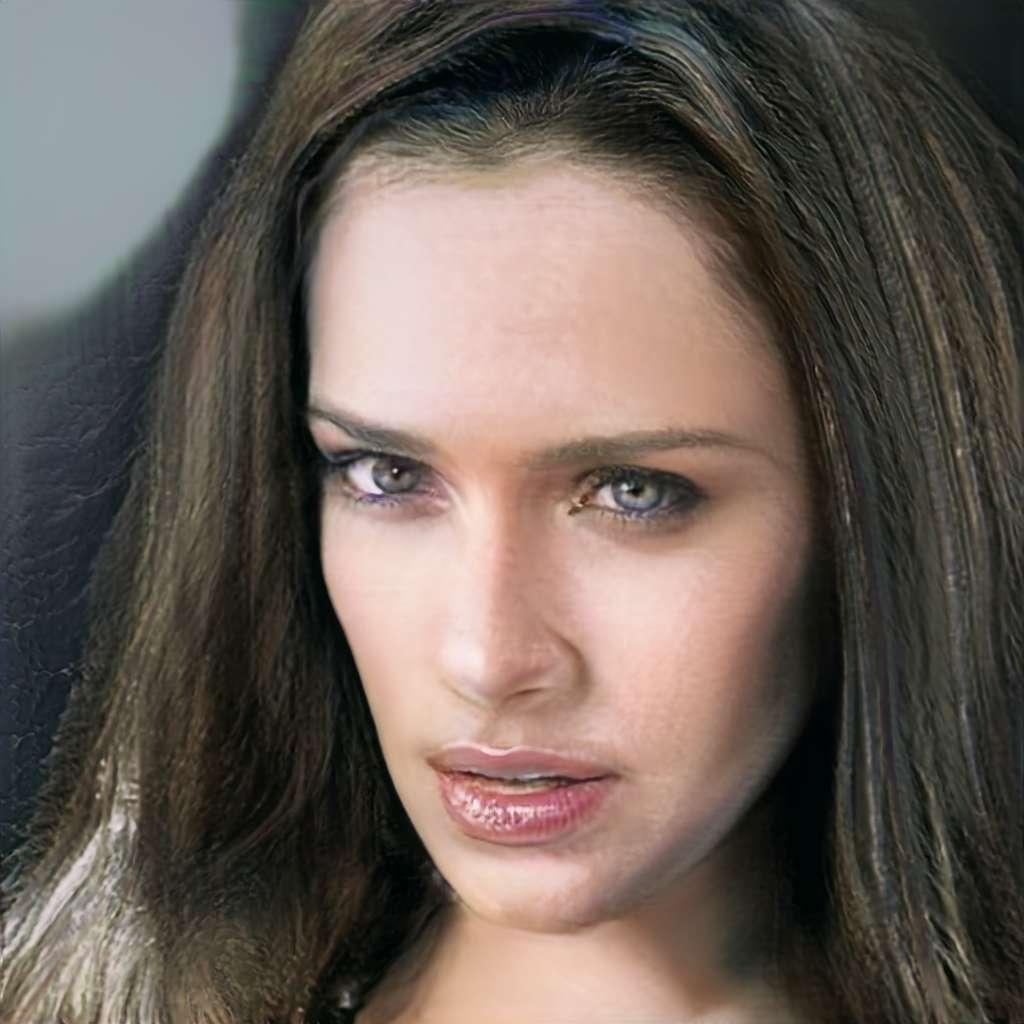
\includegraphics[width=\pganw]{figures/pgan/49_base_iso_base.jpg} &
\unreal{
\includegraphics[width=\pganw]{figures/pgan/48_base_iso_reject.jpg}} &
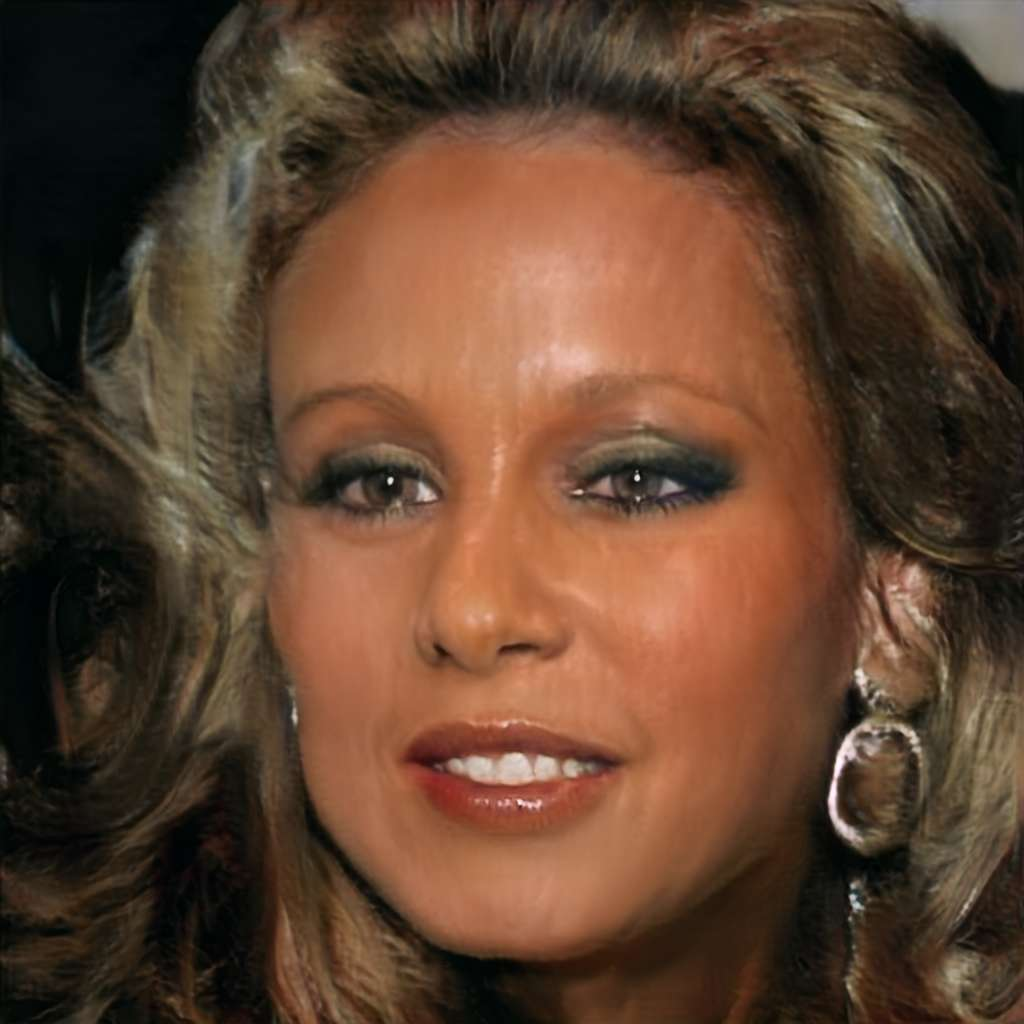
\includegraphics[width=\pganw]{figures/pgan/49_base_iso_reject.jpg} &
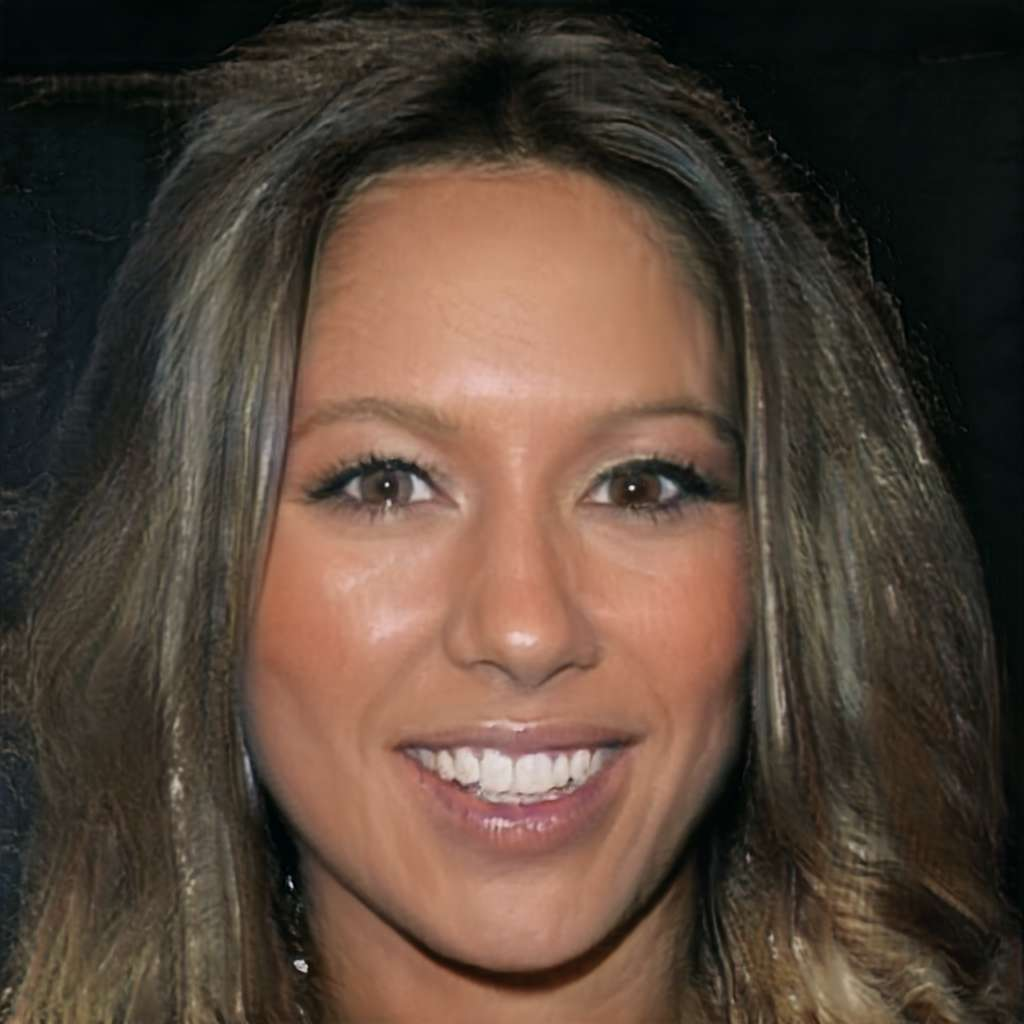
\includegraphics[width=\pganw]{figures/pgan/48_base_iso_MH.jpg} &
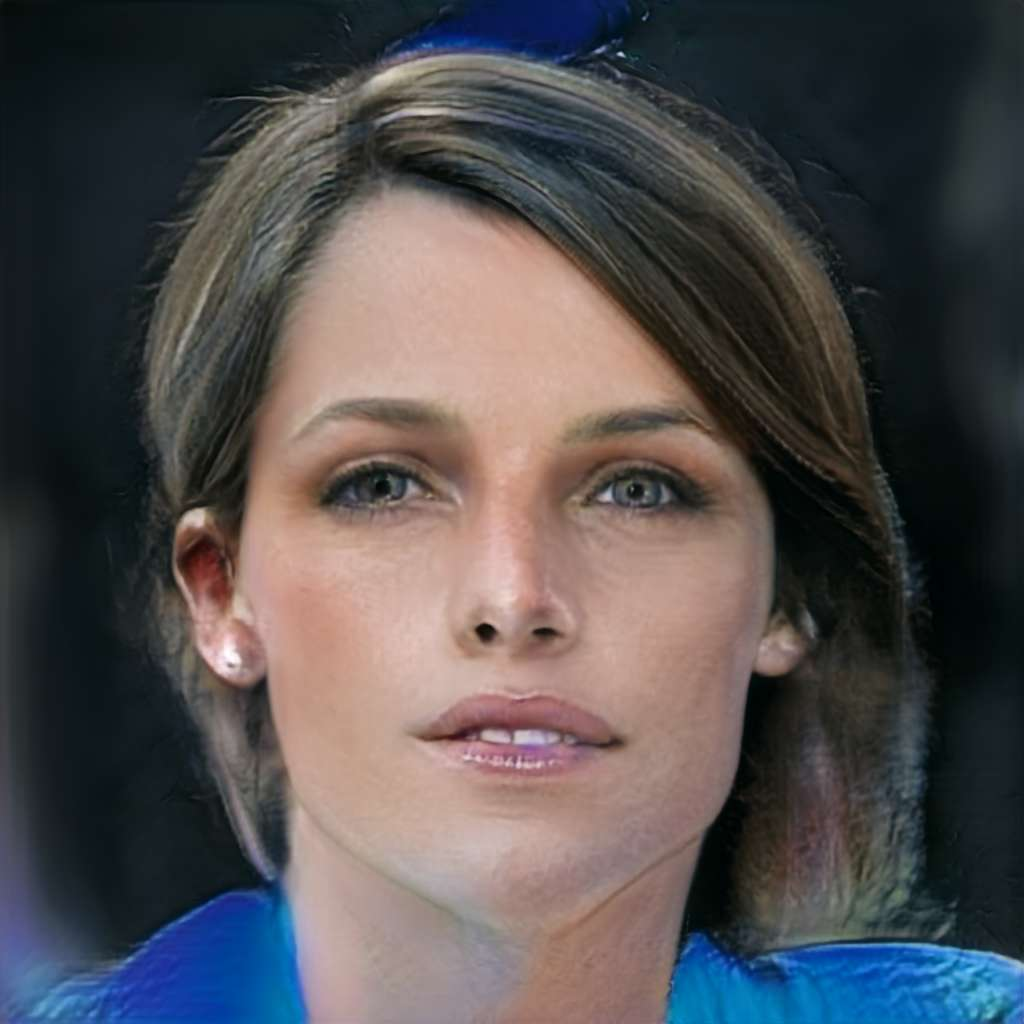
\includegraphics[width=\pganw]{figures/pgan/49_base_iso_MH.jpg} \\
\unreal{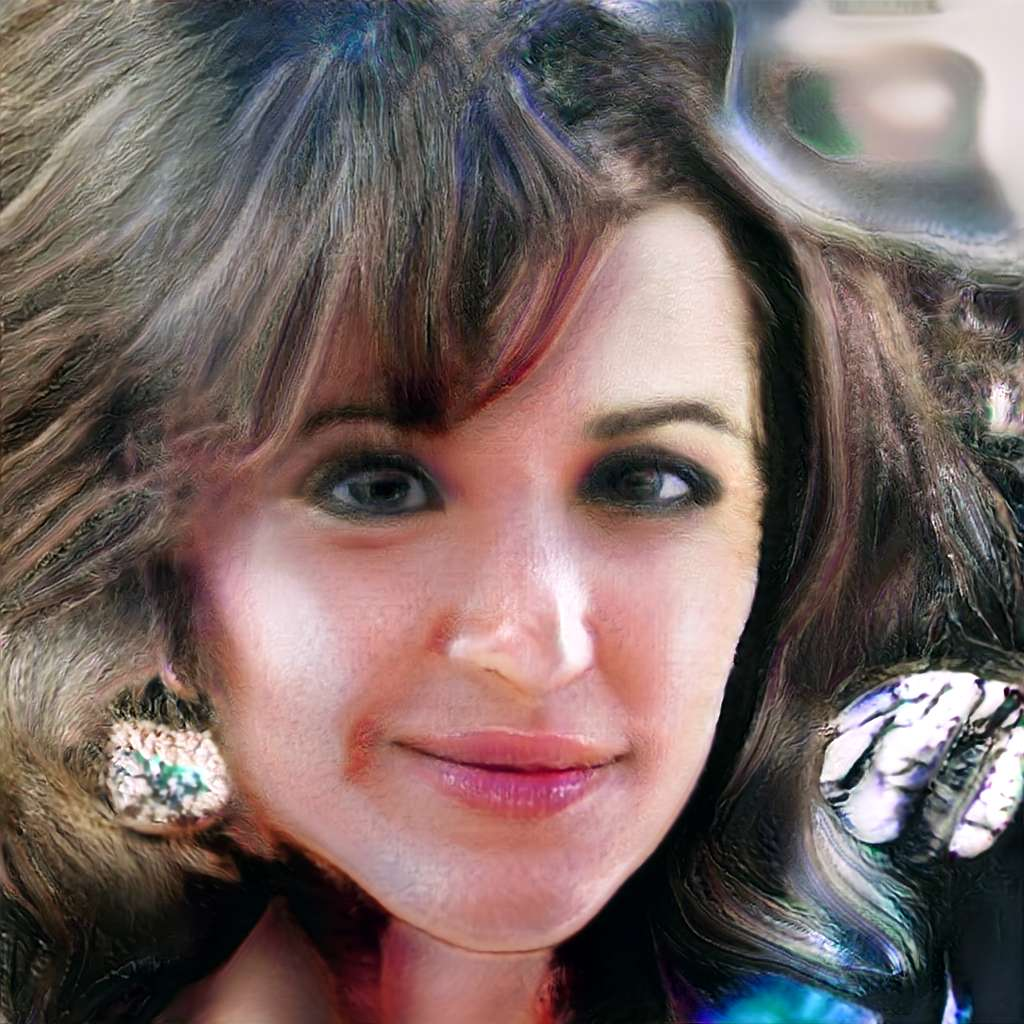
\includegraphics[width=\pganw]{figures/pgan/50_base_iso_base.jpg}} &
\unreal{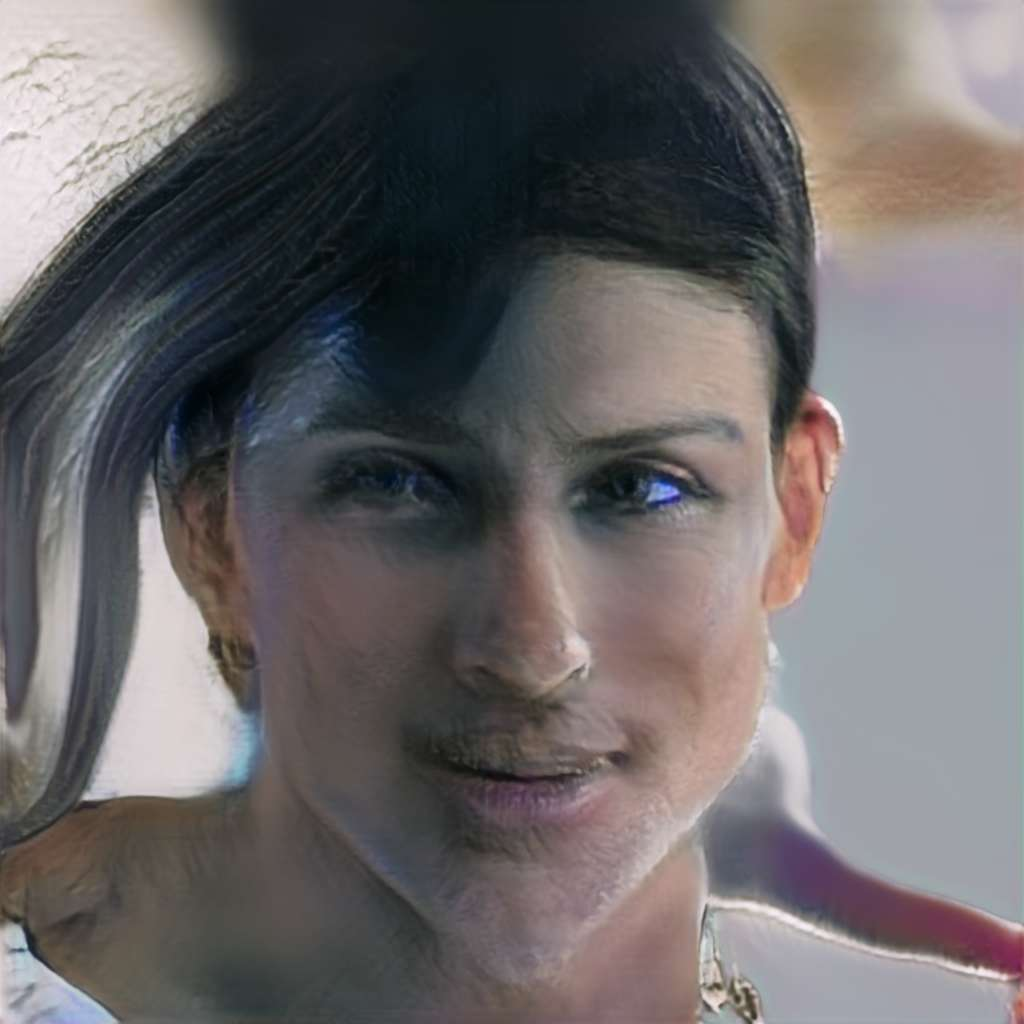
\includegraphics[width=\pganw]{figures/pgan/51_base_iso_base.jpg}} &
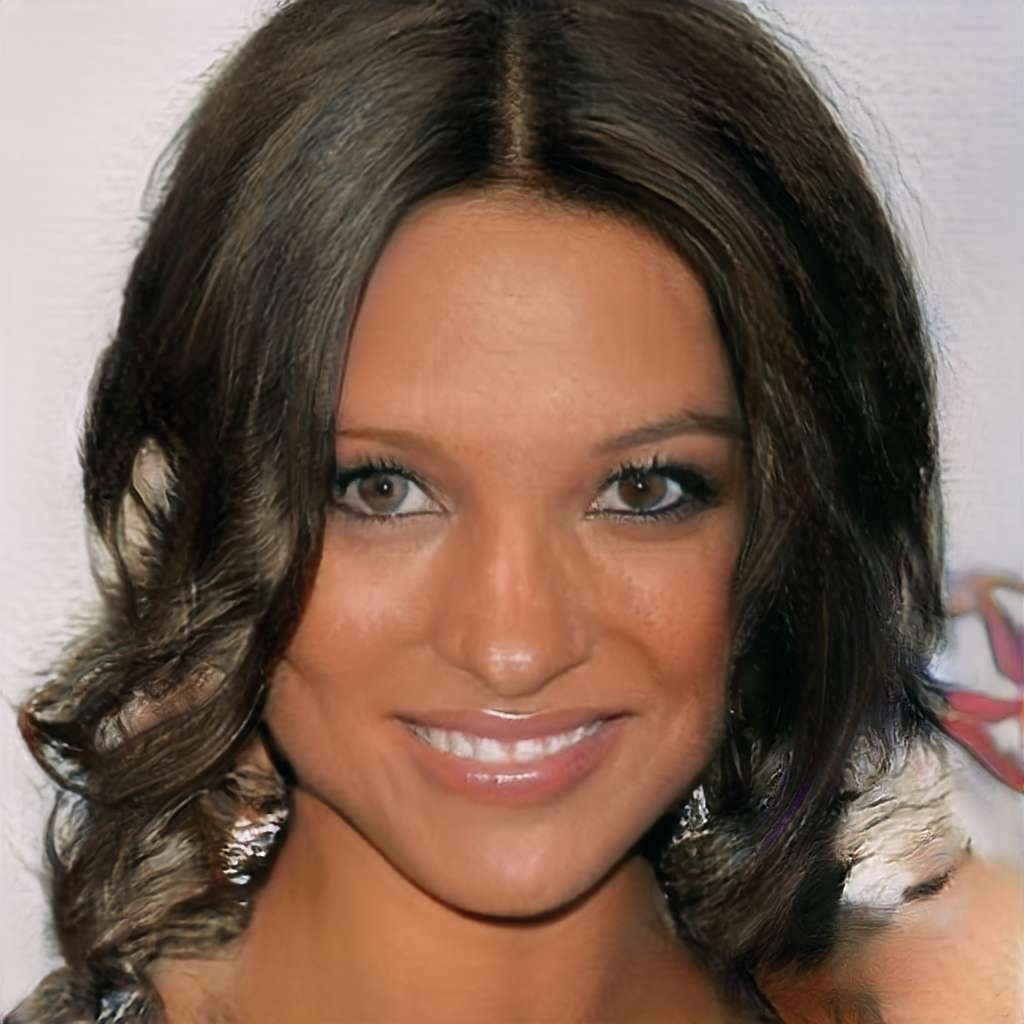
\includegraphics[width=\pganw]{figures/pgan/50_base_iso_reject.jpg} &
\unreal{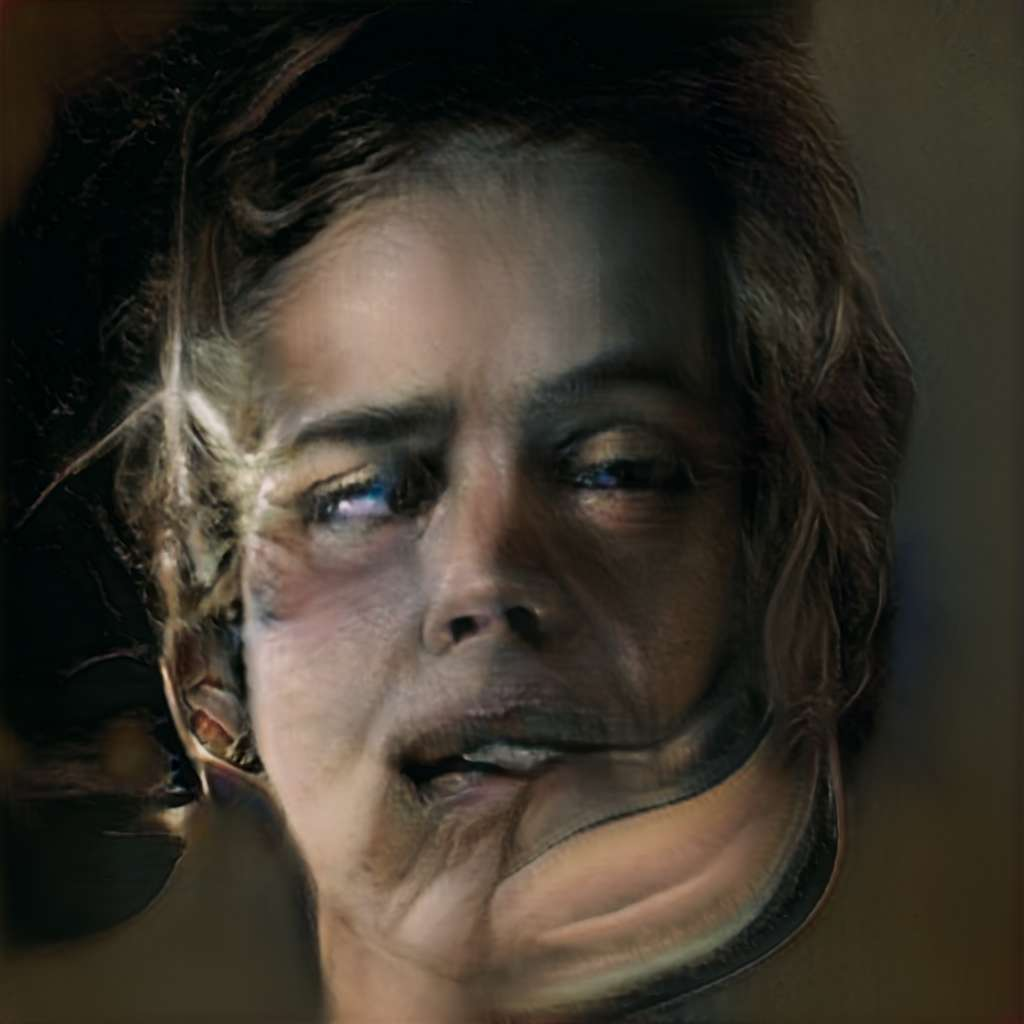
\includegraphics[width=\pganw]{figures/pgan/51_base_iso_reject.jpg}} &
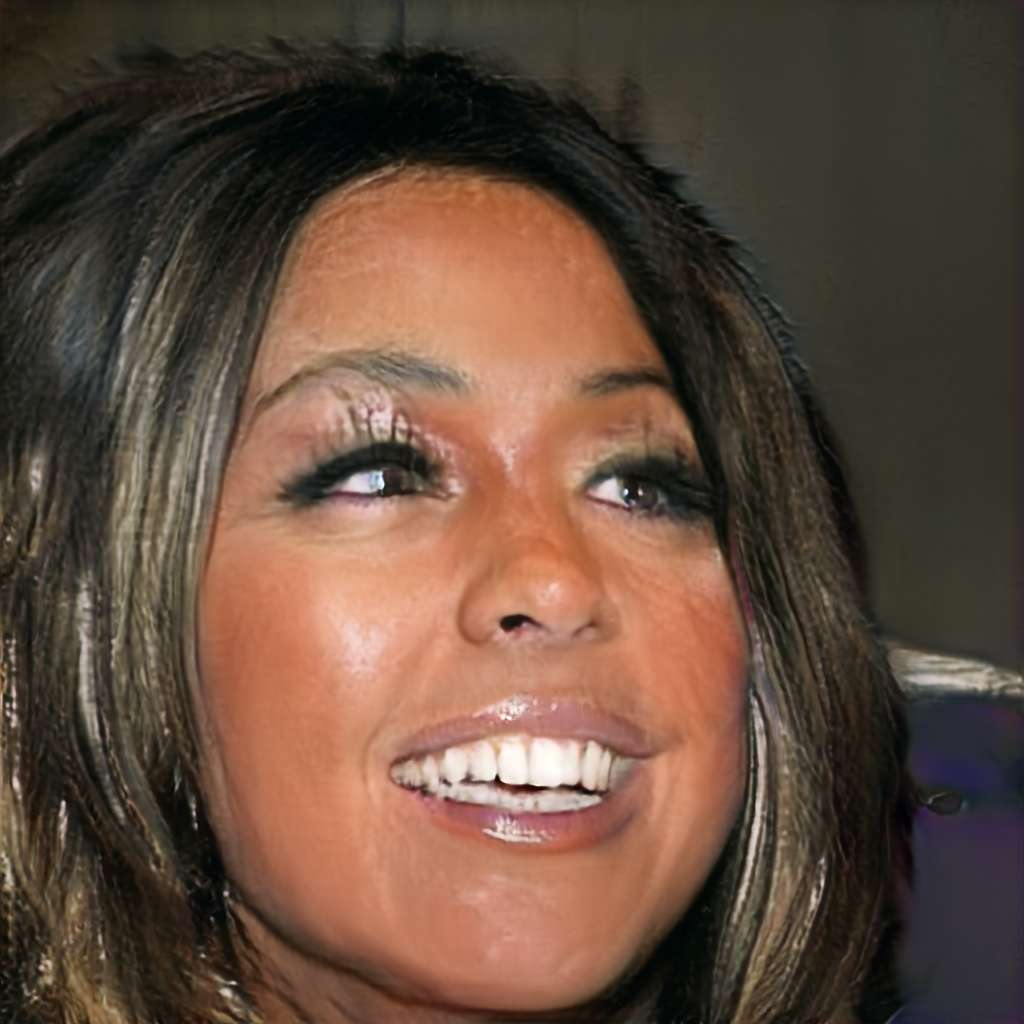
\includegraphics[width=\pganw]{figures/pgan/50_base_iso_MH.jpg} &
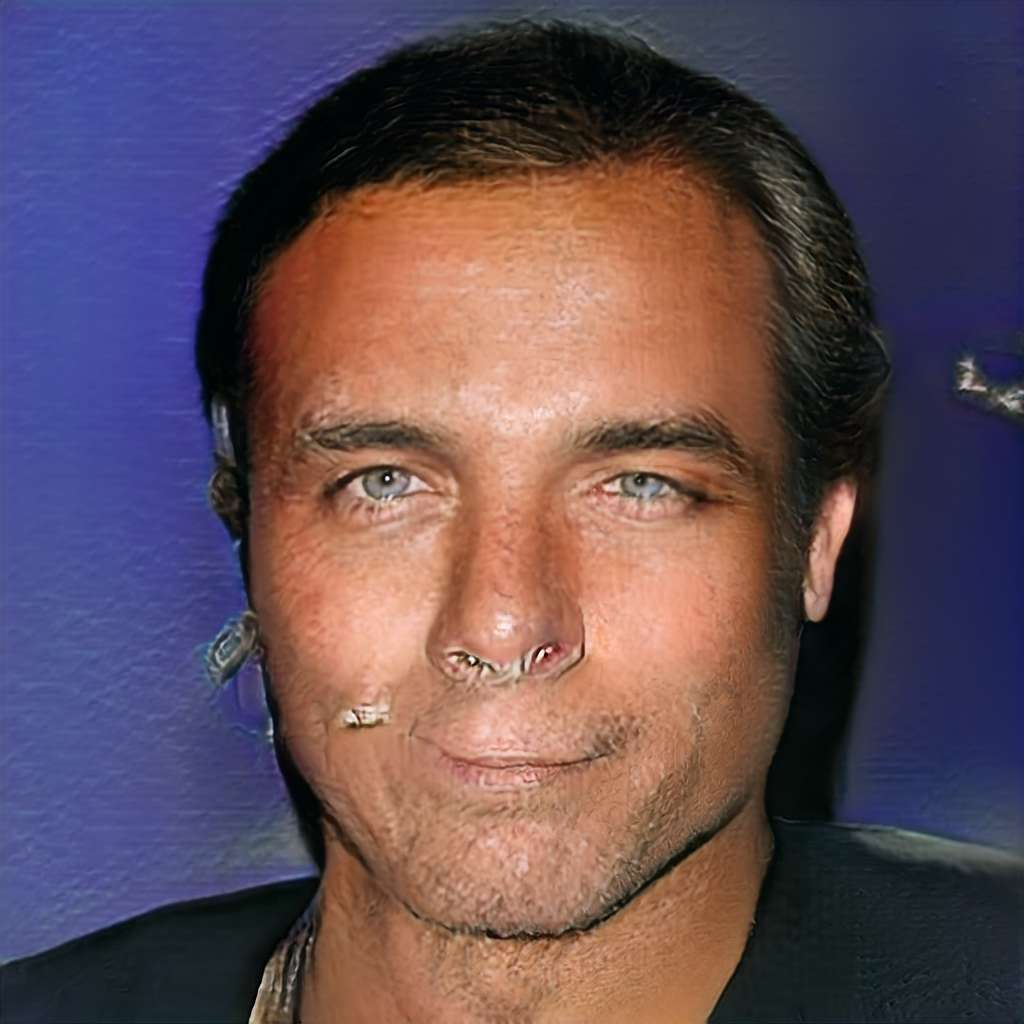
\includegraphics[width=\pganw]{figures/pgan/51_base_iso_MH.jpg} \\
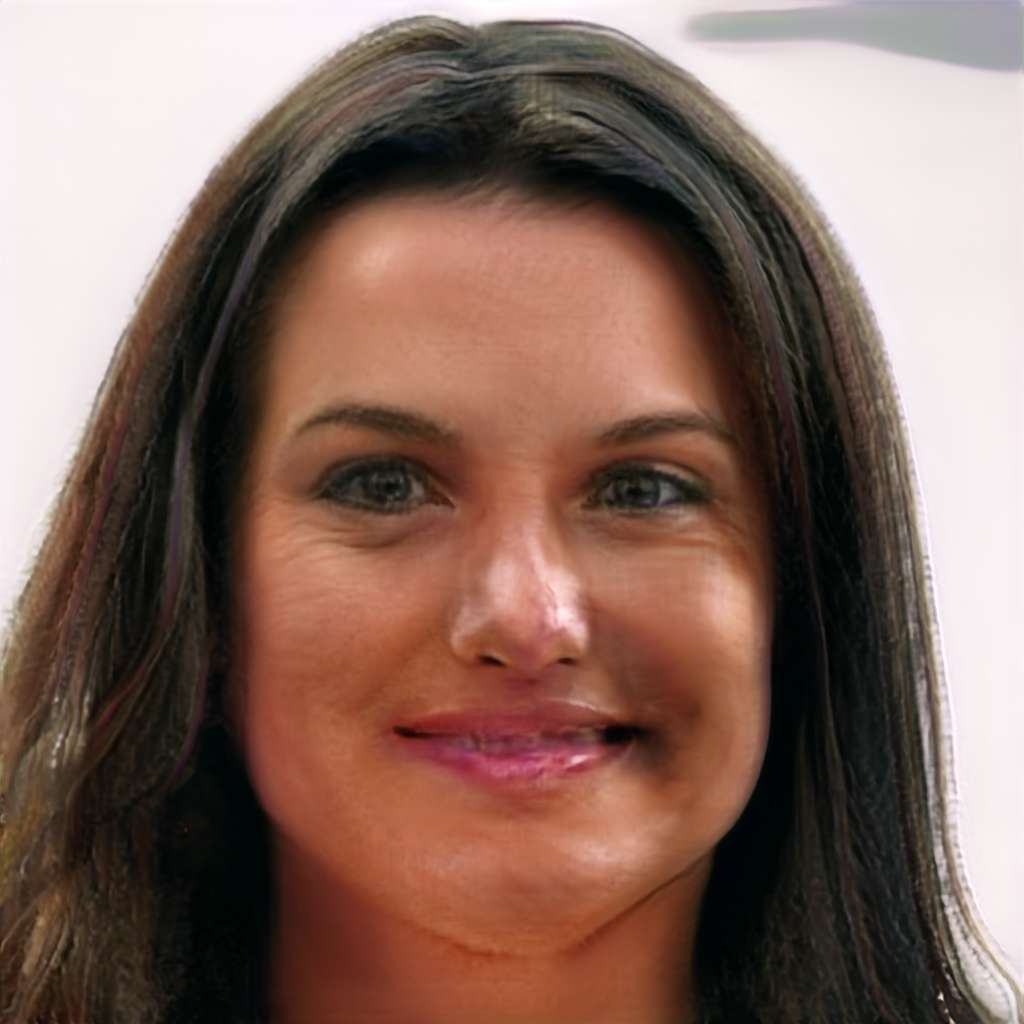
\includegraphics[width=\pganw]{figures/pgan/52_base_iso_base.jpg} &
\unreal{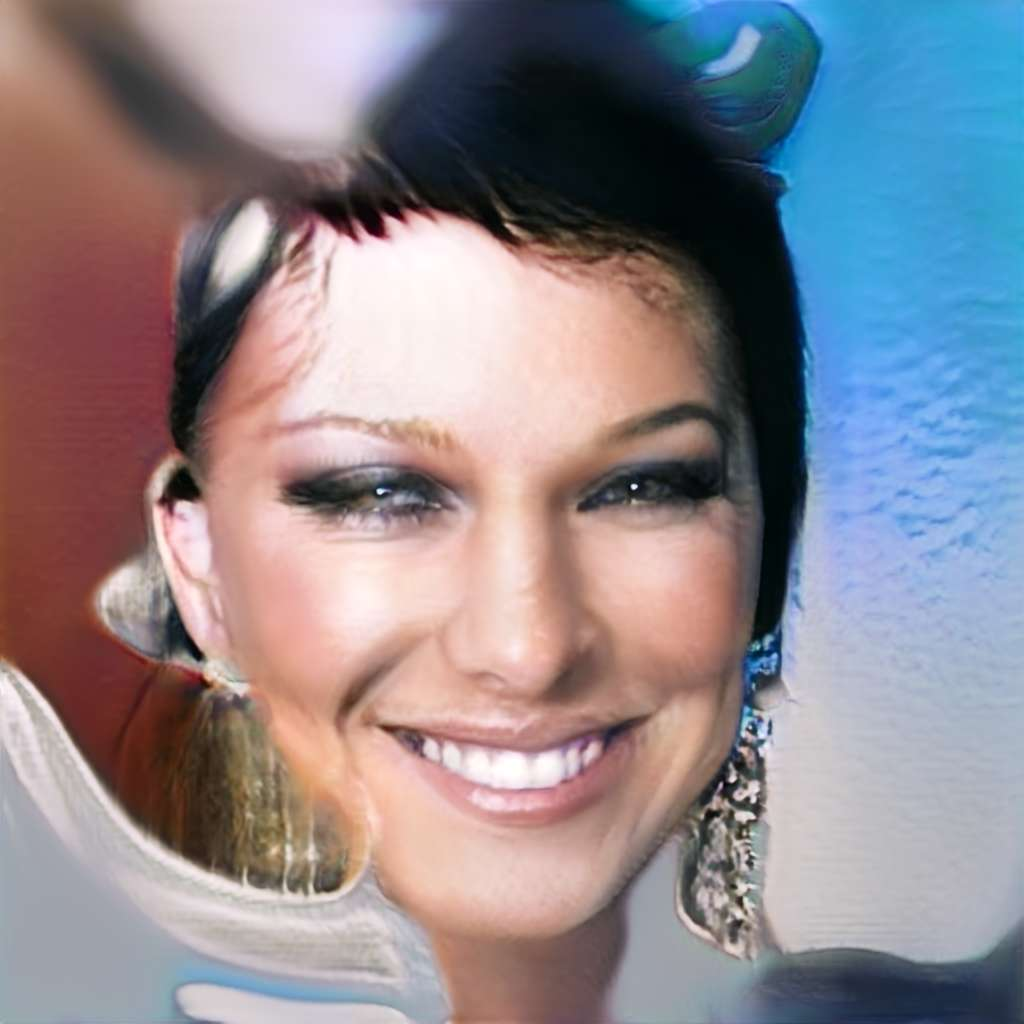
\includegraphics[width=\pganw]{figures/pgan/53_base_iso_base.jpg}} &
\unreal{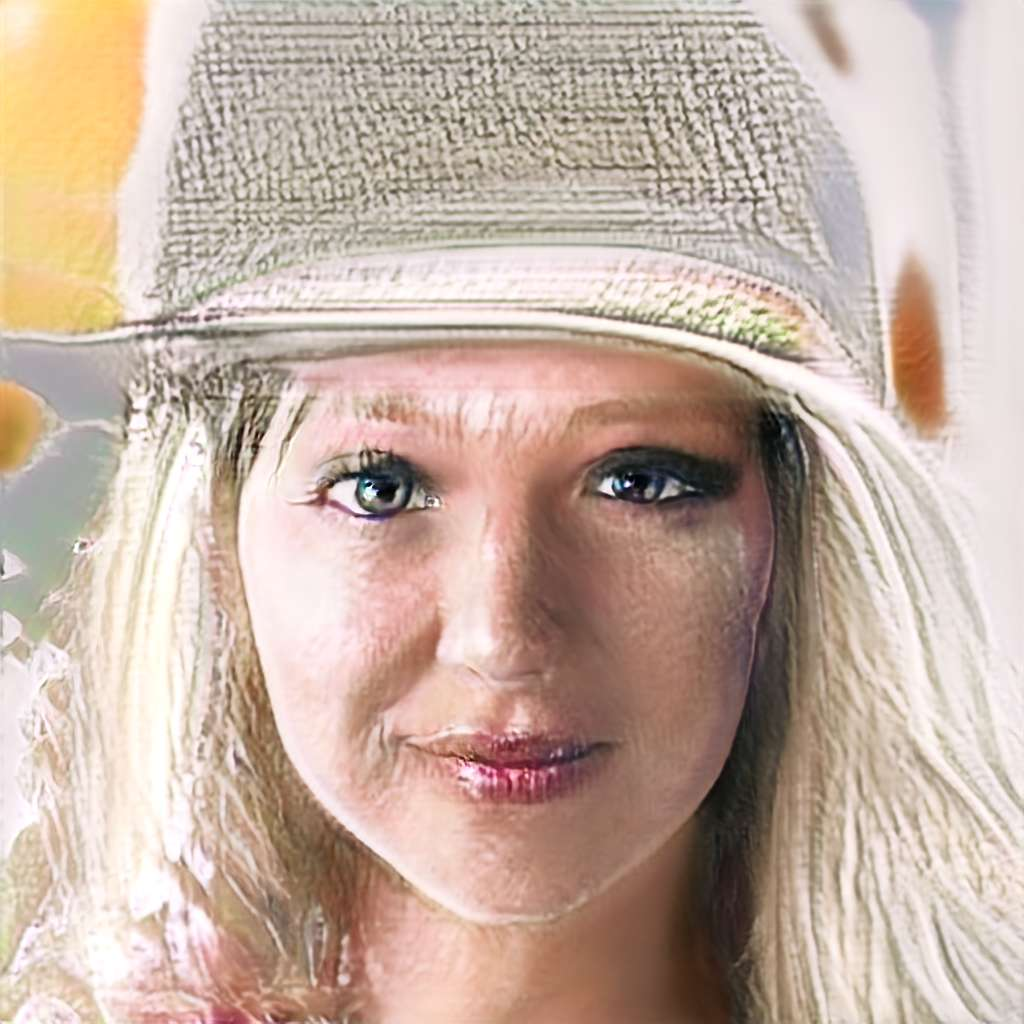
\includegraphics[width=\pganw]{figures/pgan/52_base_iso_reject.jpg}} &
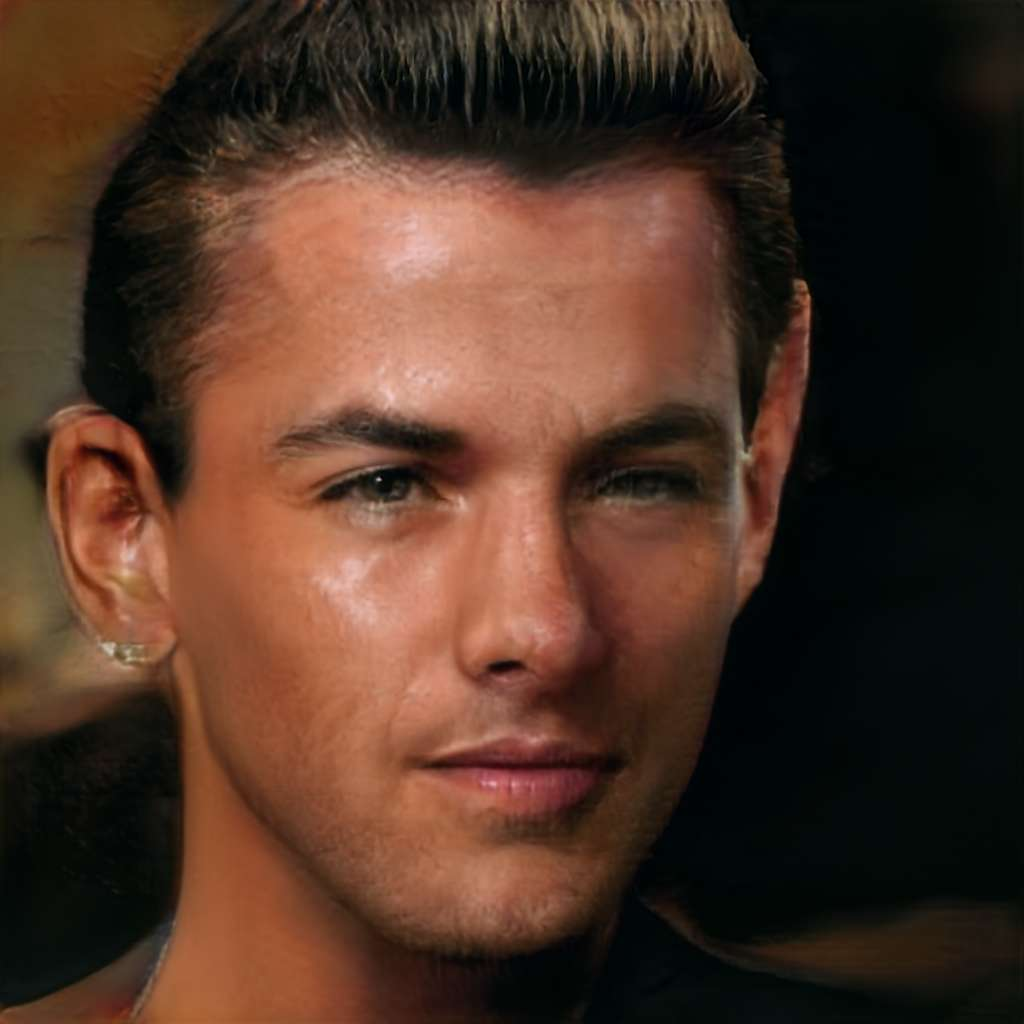
\includegraphics[width=\pganw]{figures/pgan/53_base_iso_reject.jpg} &
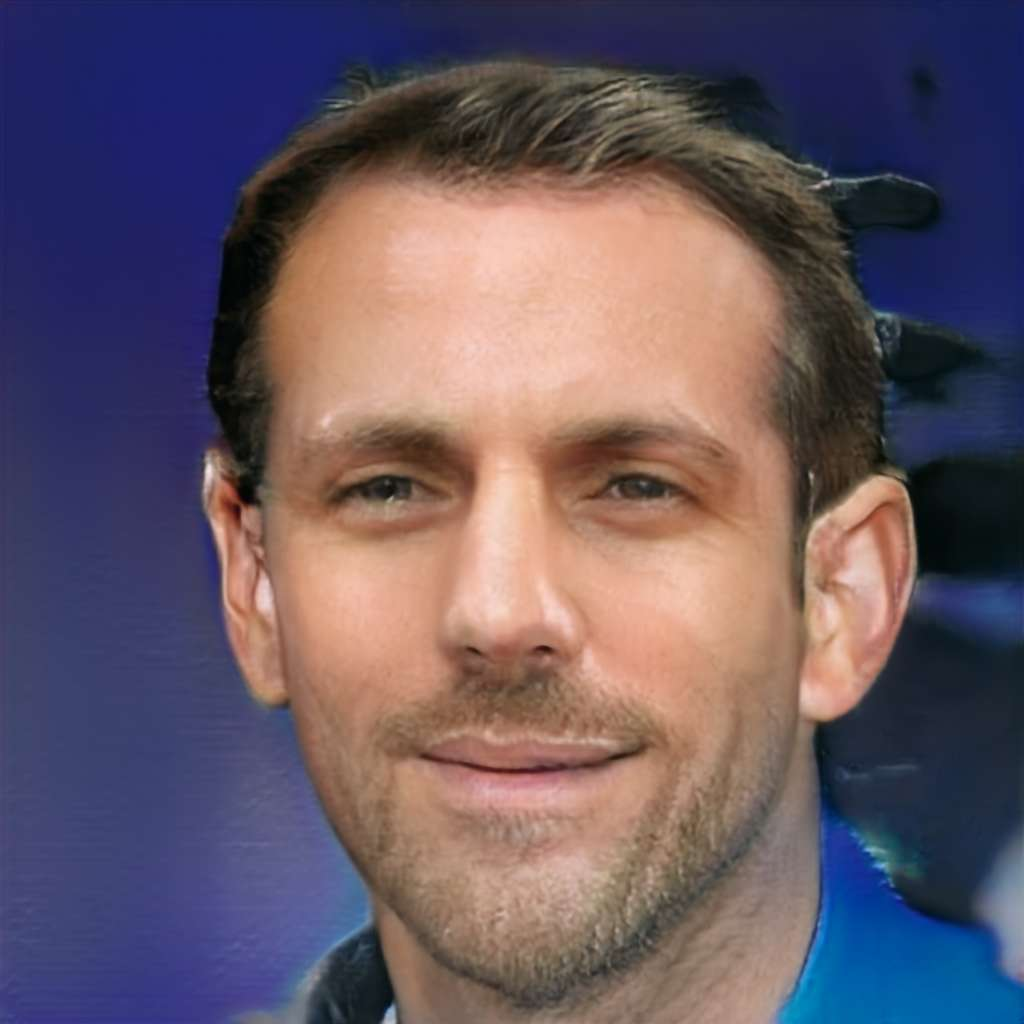
\includegraphics[width=\pganw]{figures/pgan/52_base_iso_MH.jpg} &
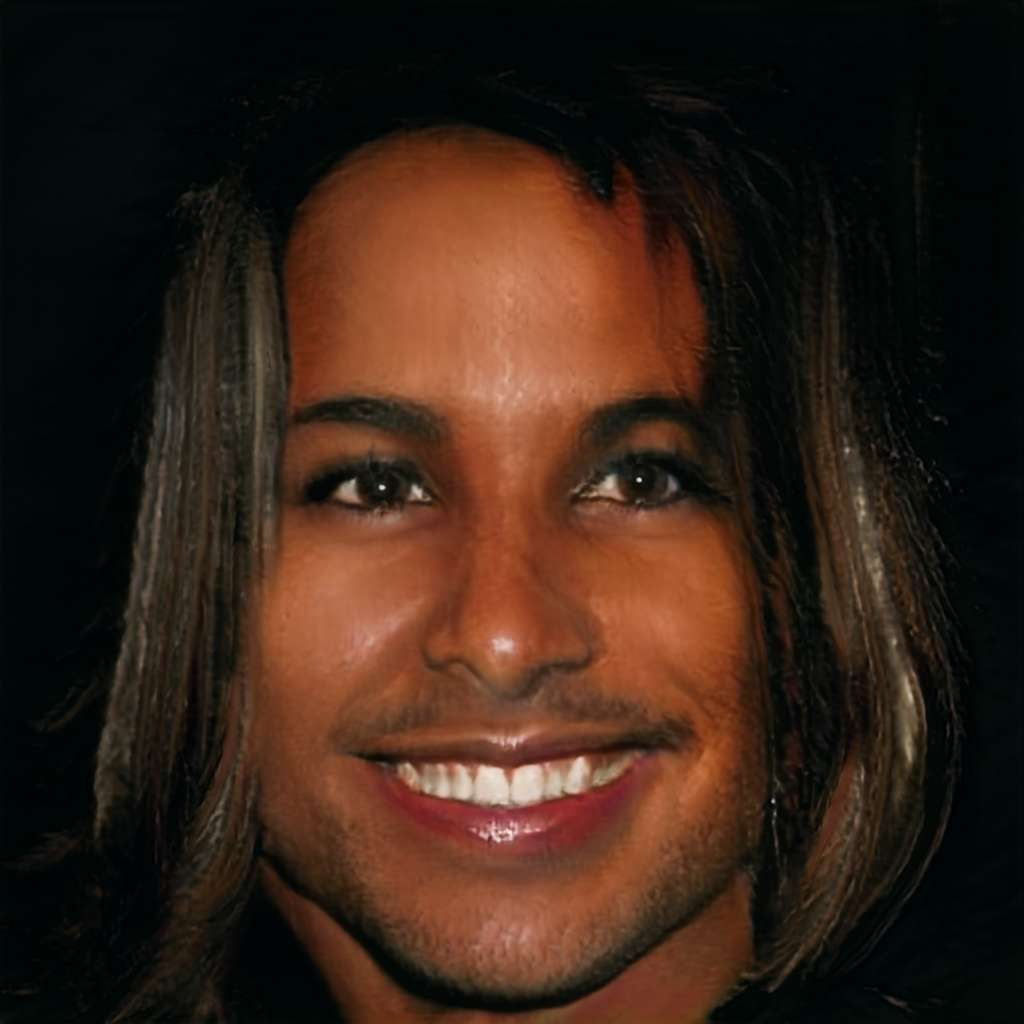
\includegraphics[width=\pganw]{figures/pgan/53_base_iso_MH.jpg} \\
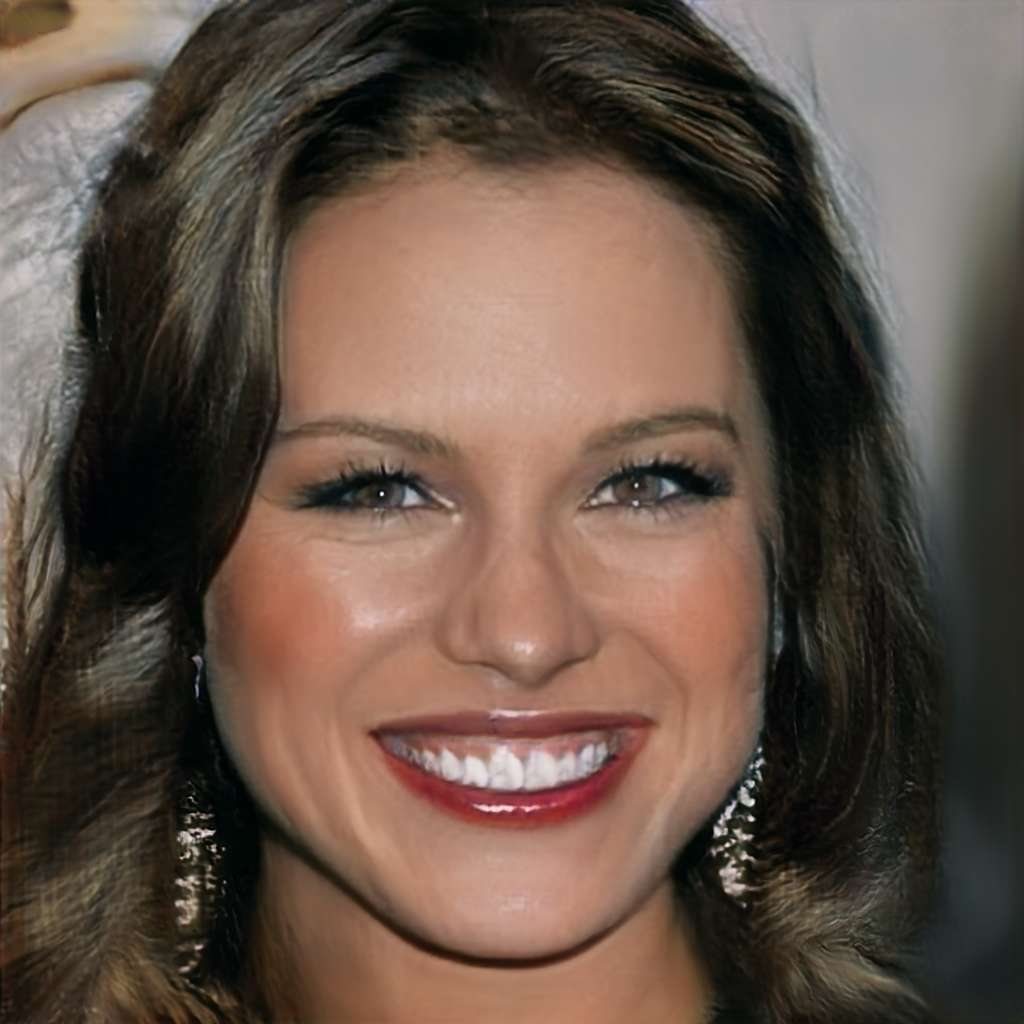
\includegraphics[width=\pganw]{figures/pgan/54_base_iso_base.jpg} &
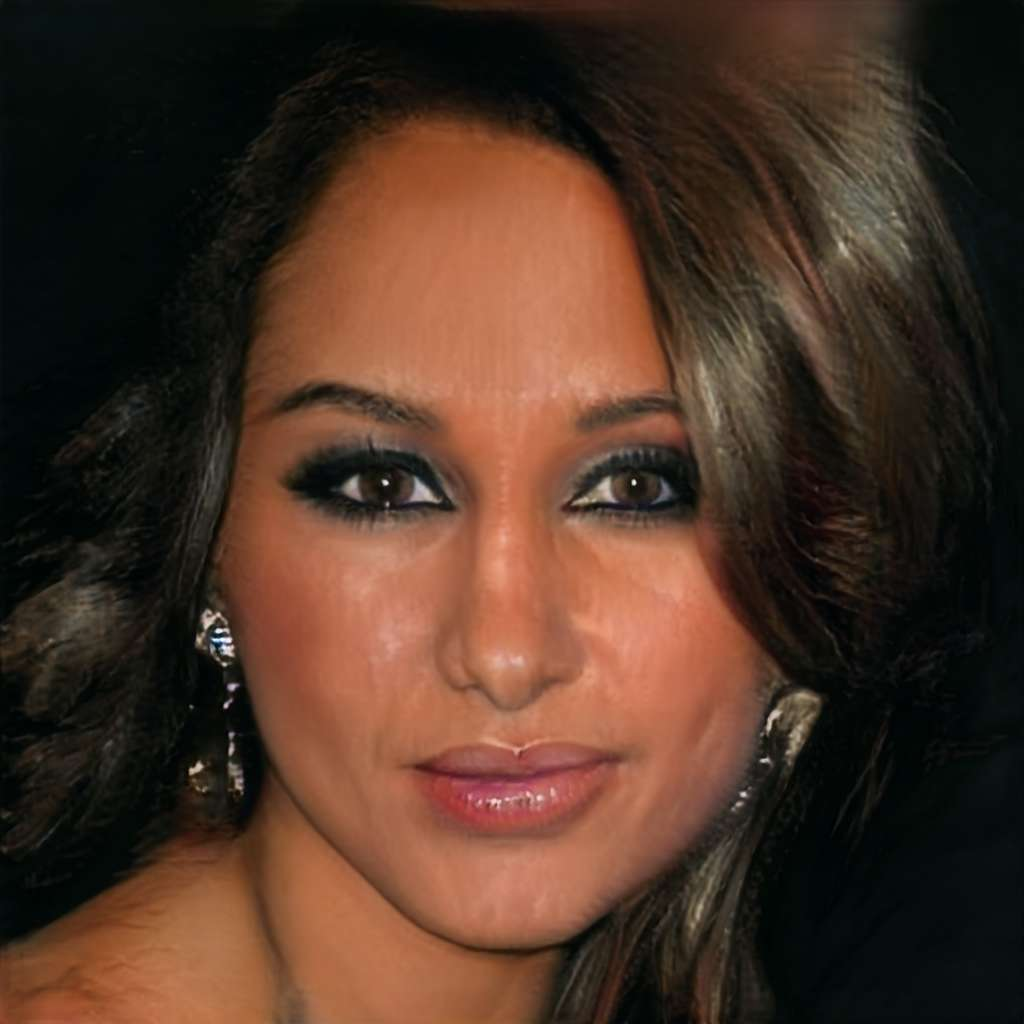
\includegraphics[width=\pganw]{figures/pgan/55_base_iso_base.jpg} &
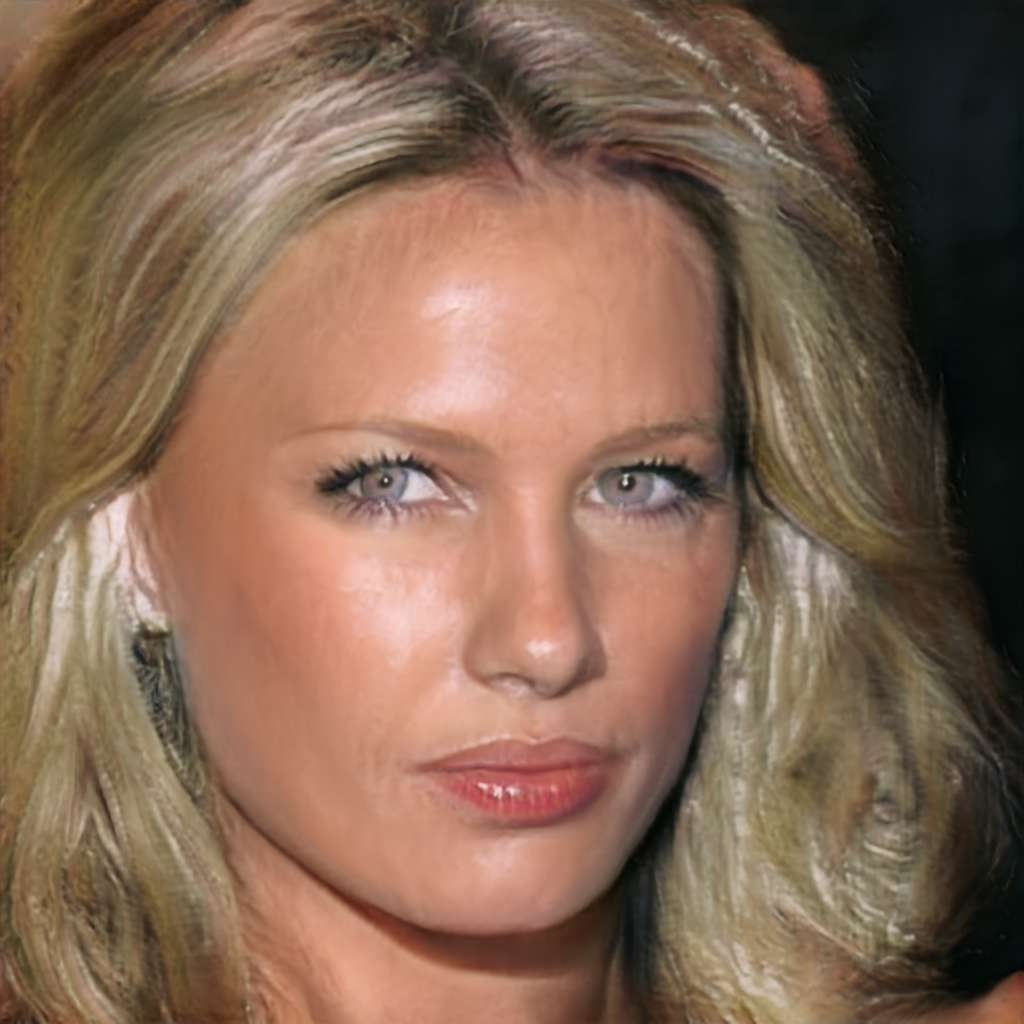
\includegraphics[width=\pganw]{figures/pgan/54_base_iso_reject.jpg} &
\unreal{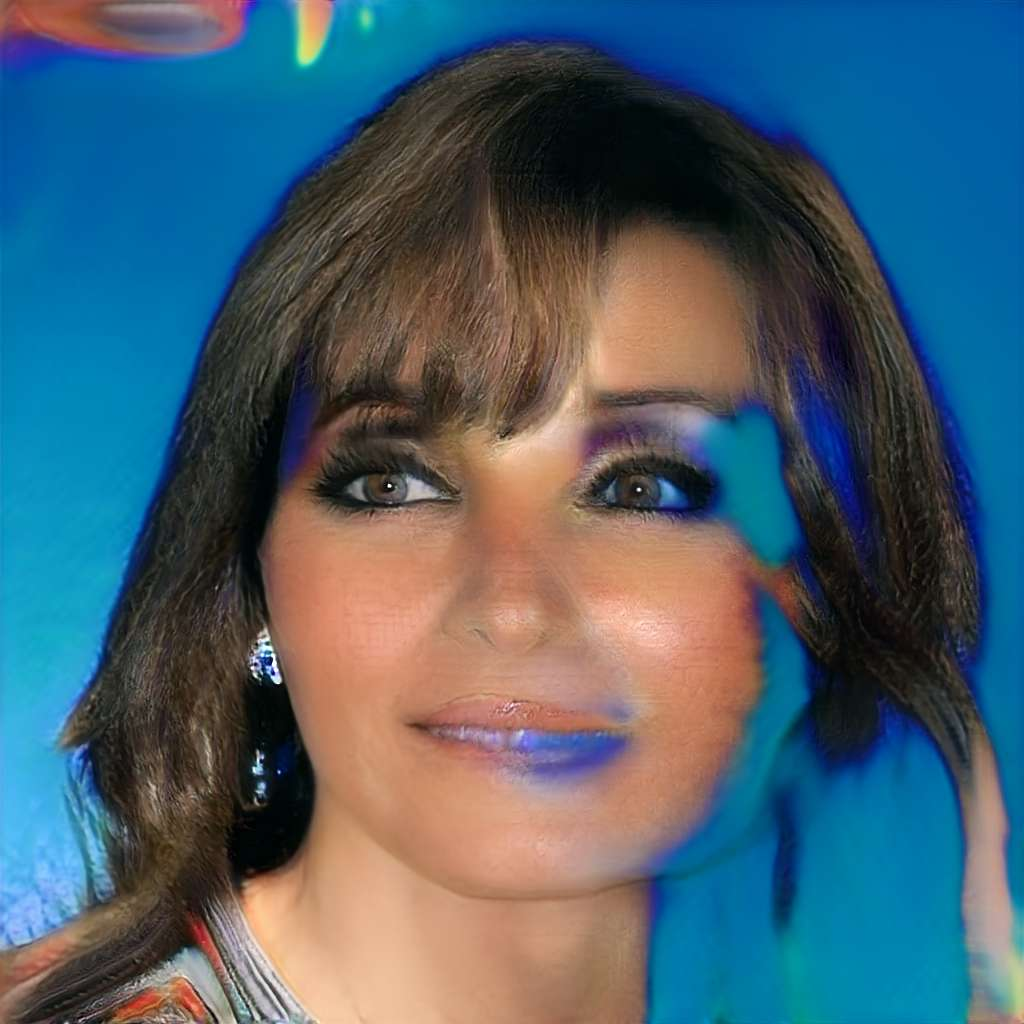
\includegraphics[width=\pganw]{figures/pgan/55_base_iso_reject.jpg}} &
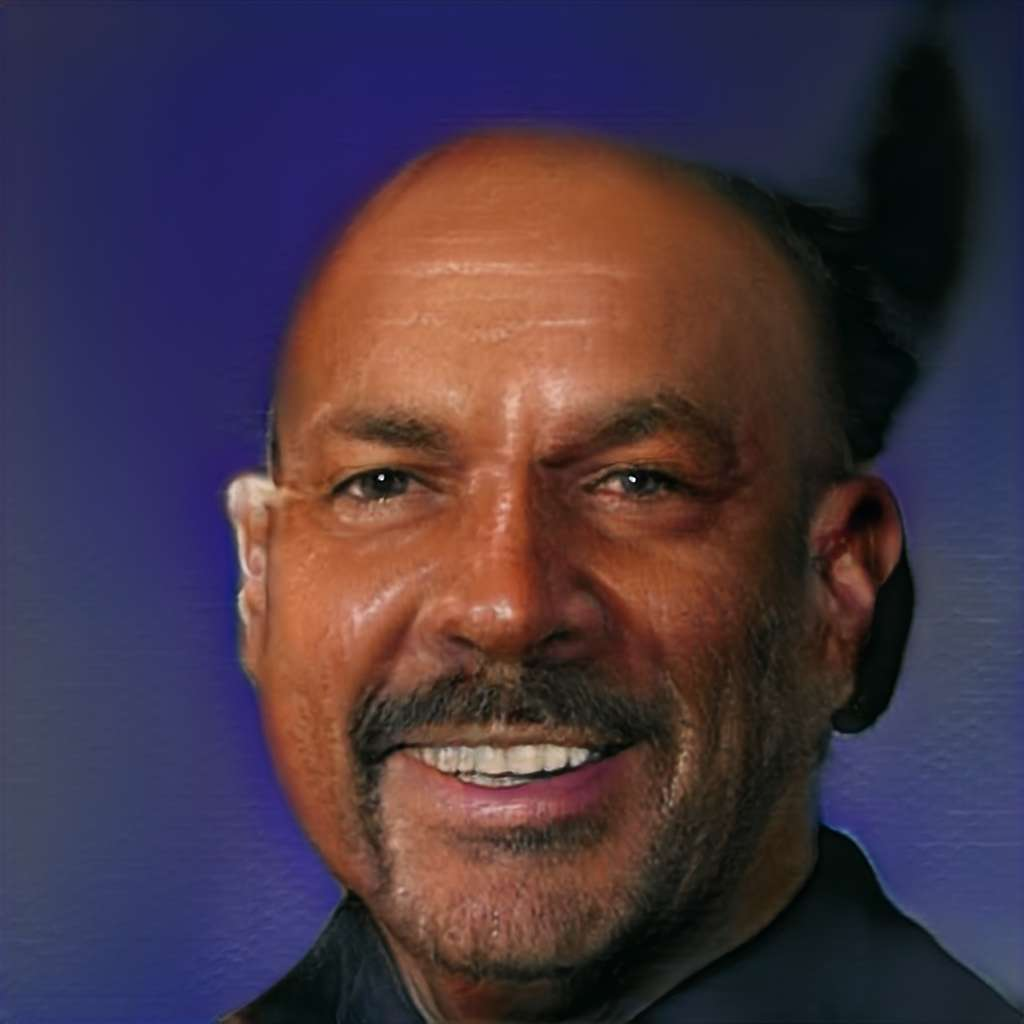
\includegraphics[width=\pganw]{figures/pgan/54_base_iso_MH.jpg} &
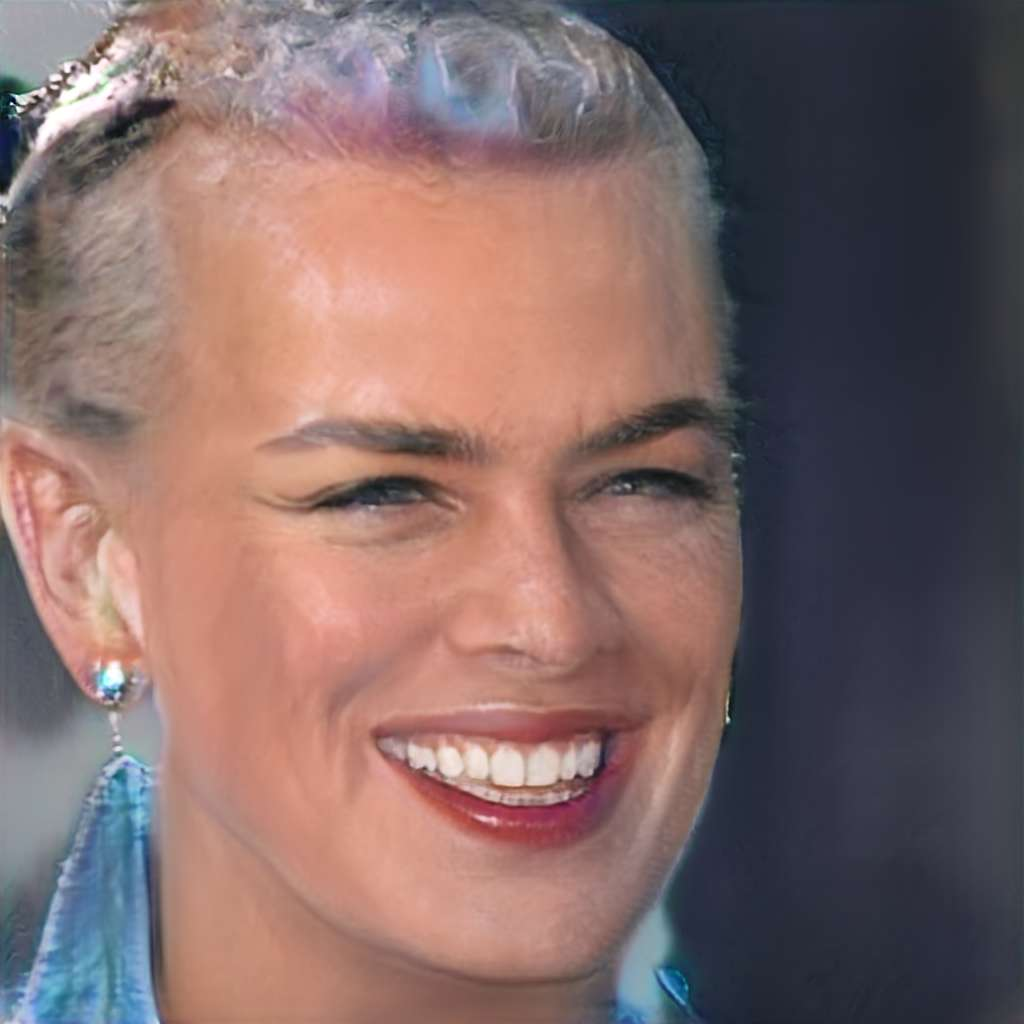
\includegraphics[width=\pganw]{figures/pgan/55_base_iso_MH.jpg} \\

\includegraphics[width=\pganw]{figures/pgan/56_base_iso_base.jpg} &
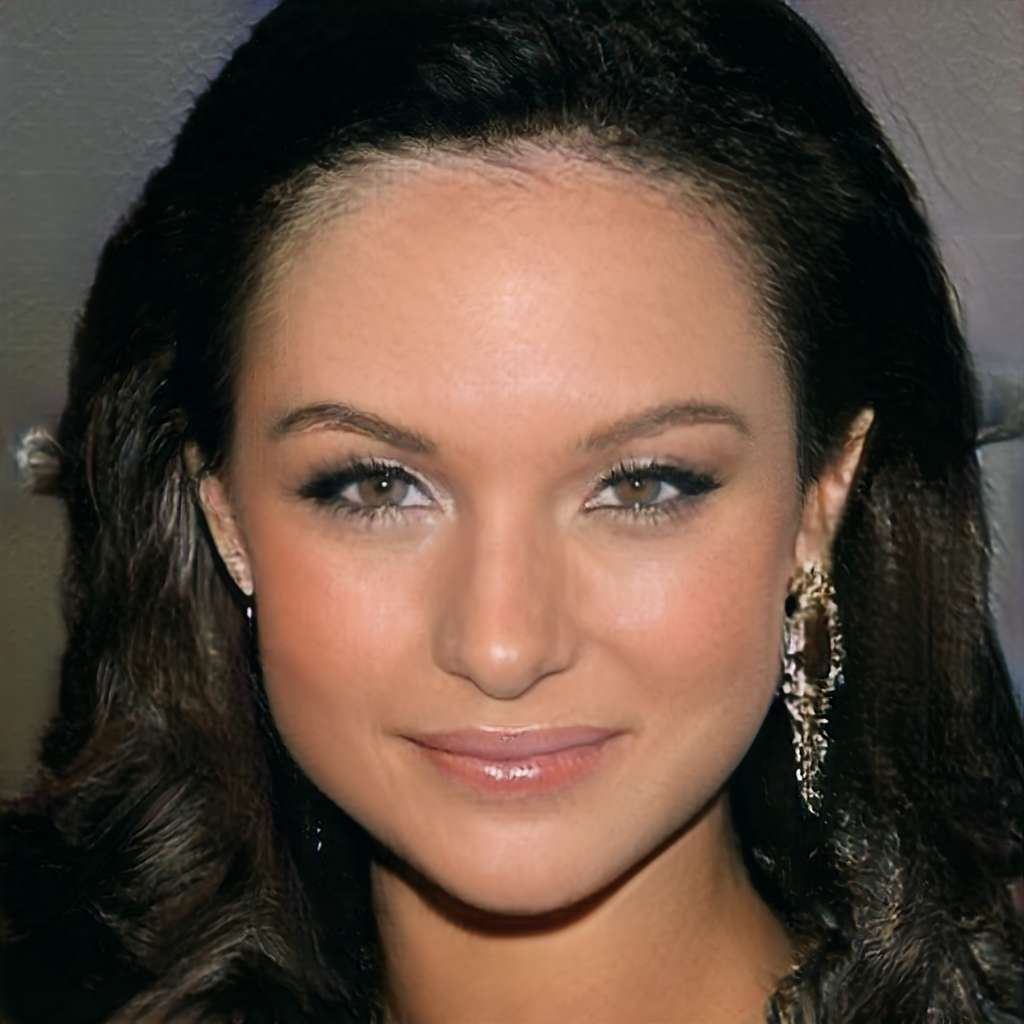
\includegraphics[width=\pganw]{figures/pgan/57_base_iso_base.jpg} &

\includegraphics[width=\pganw]{figures/pgan/56_base_iso_reject.jpg} &
\unreal{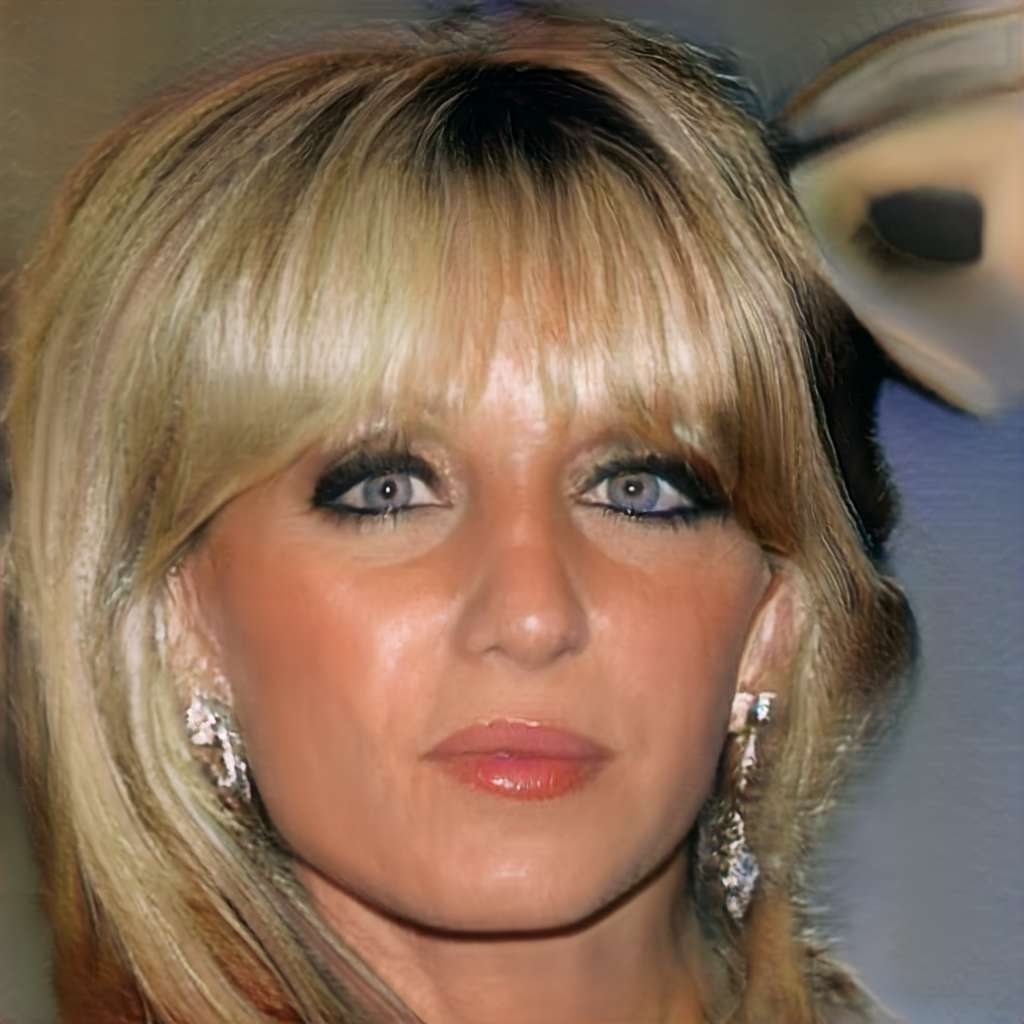
\includegraphics[width=\pganw]{figures/pgan/57_base_iso_reject.jpg}} &
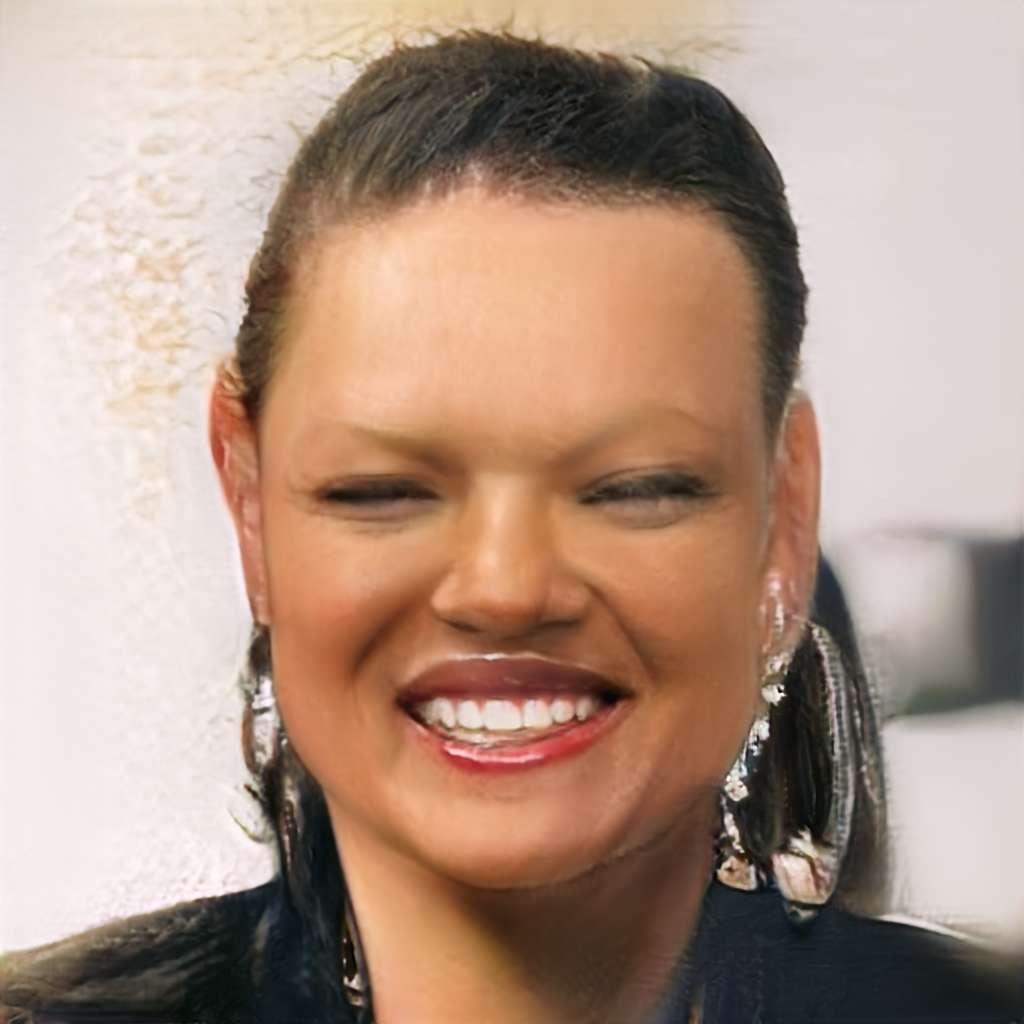
\includegraphics[width=\pganw]{figures/pgan/56_base_iso_MH.jpg} &
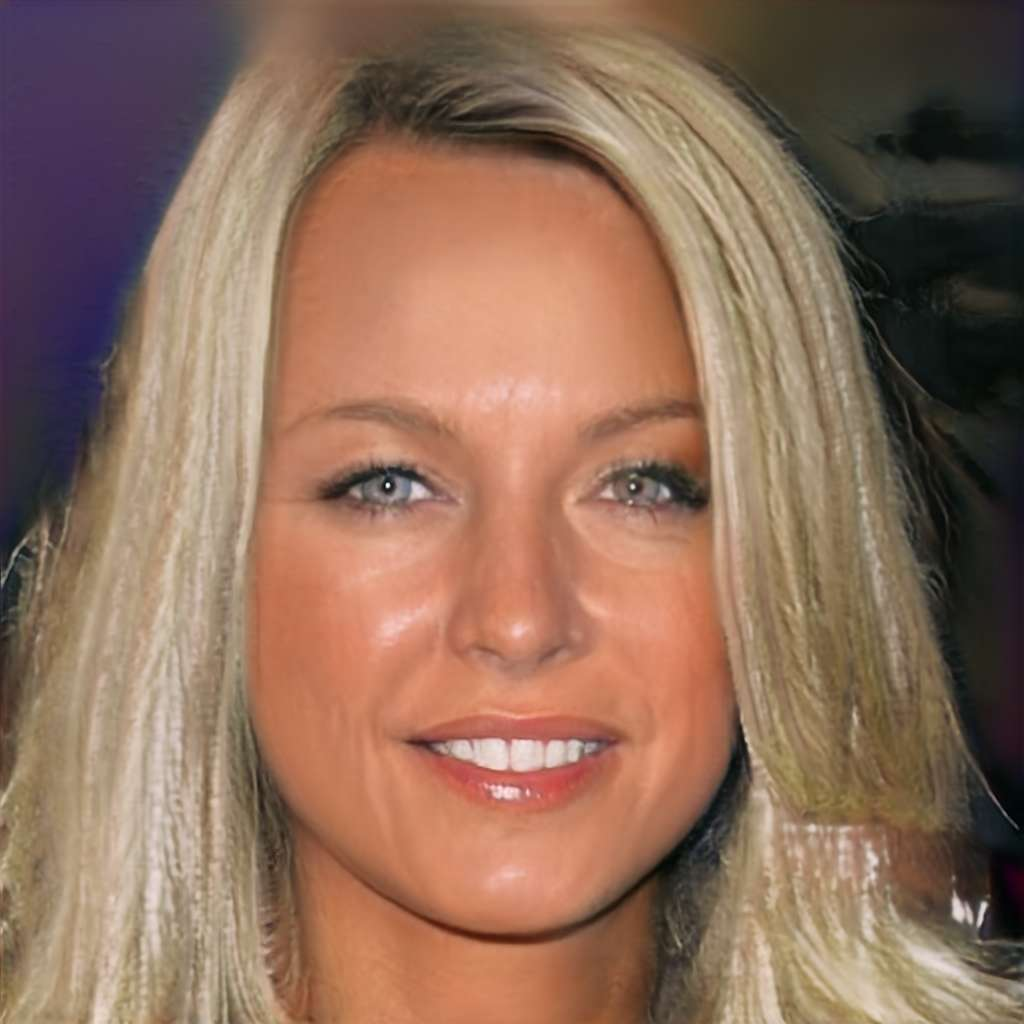
\includegraphics[width=\pganw]{figures/pgan/57_base_iso_MH.jpg} \\
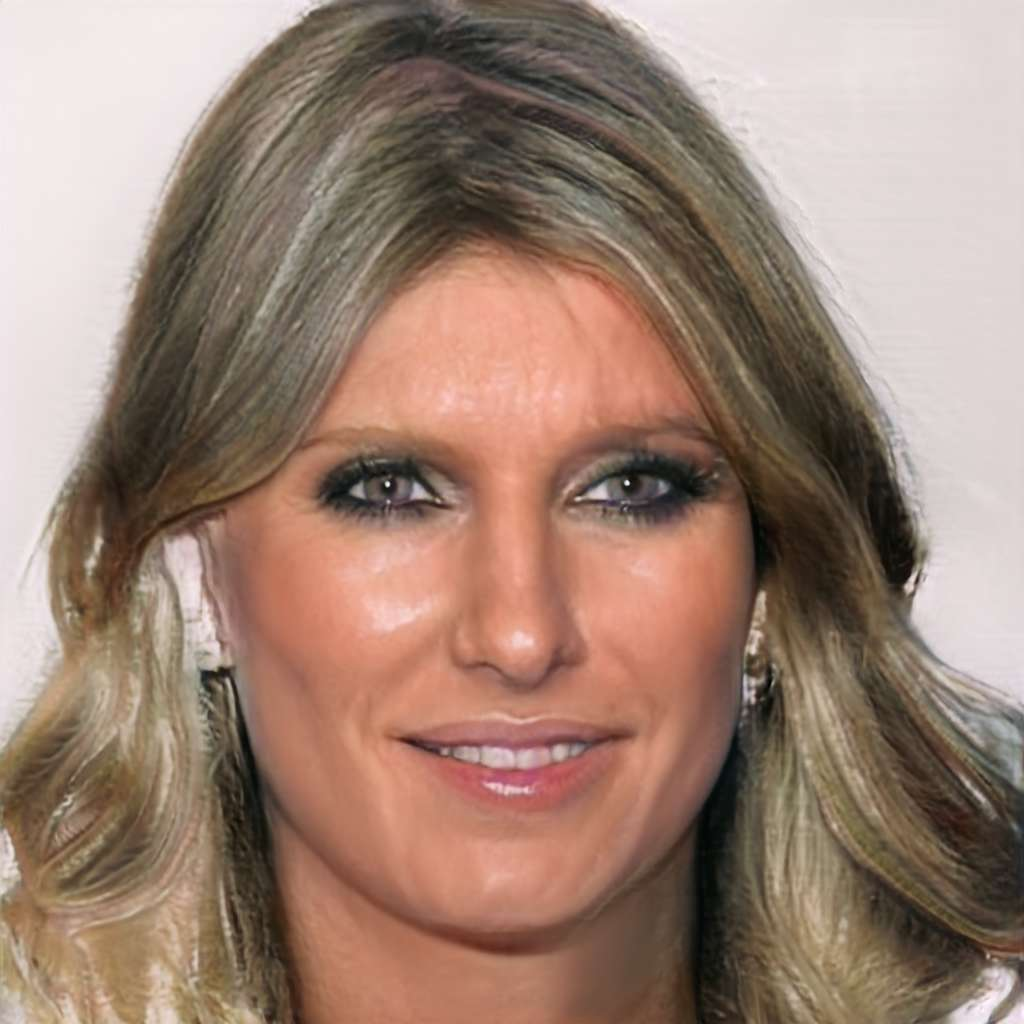
\includegraphics[width=\pganw]{figures/pgan/58_base_iso_base.jpg} &
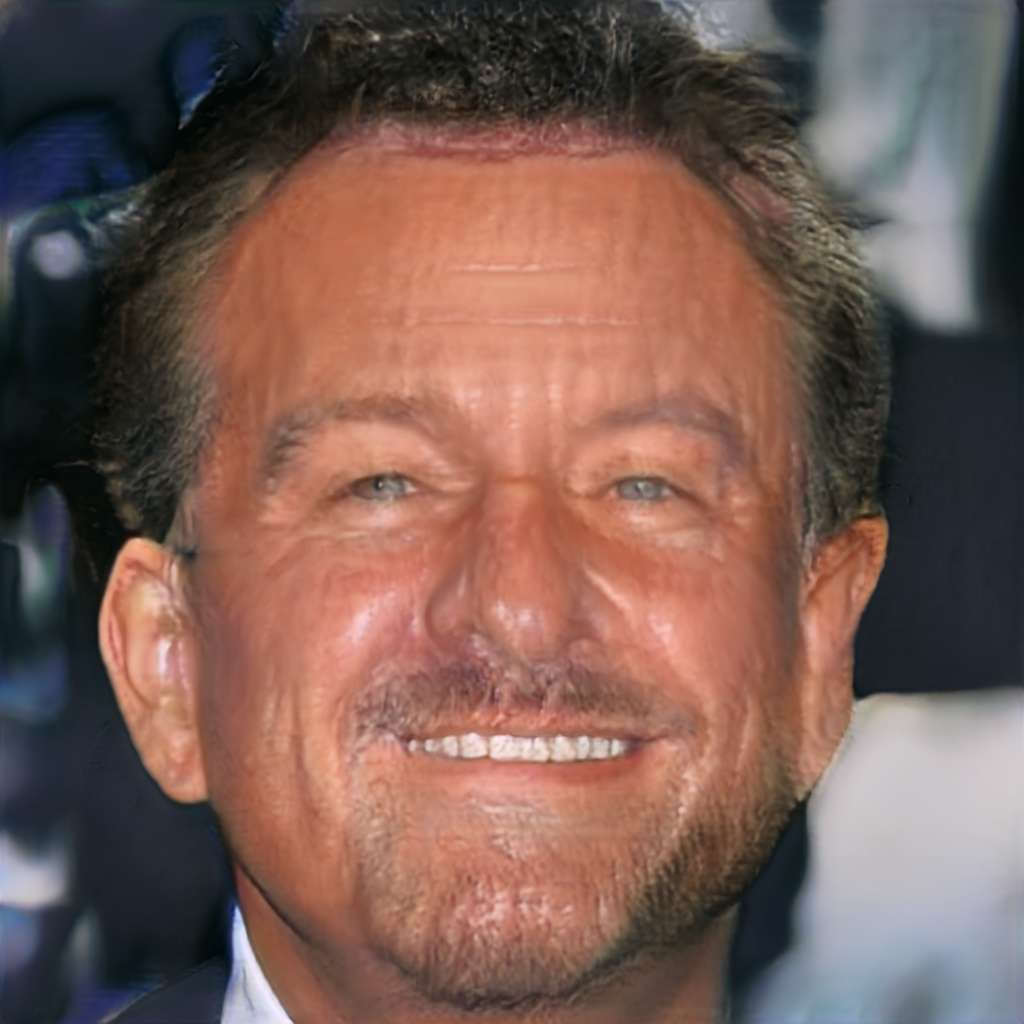
\includegraphics[width=\pganw]{figures/pgan/59_base_iso_base.jpg} &
\unreal{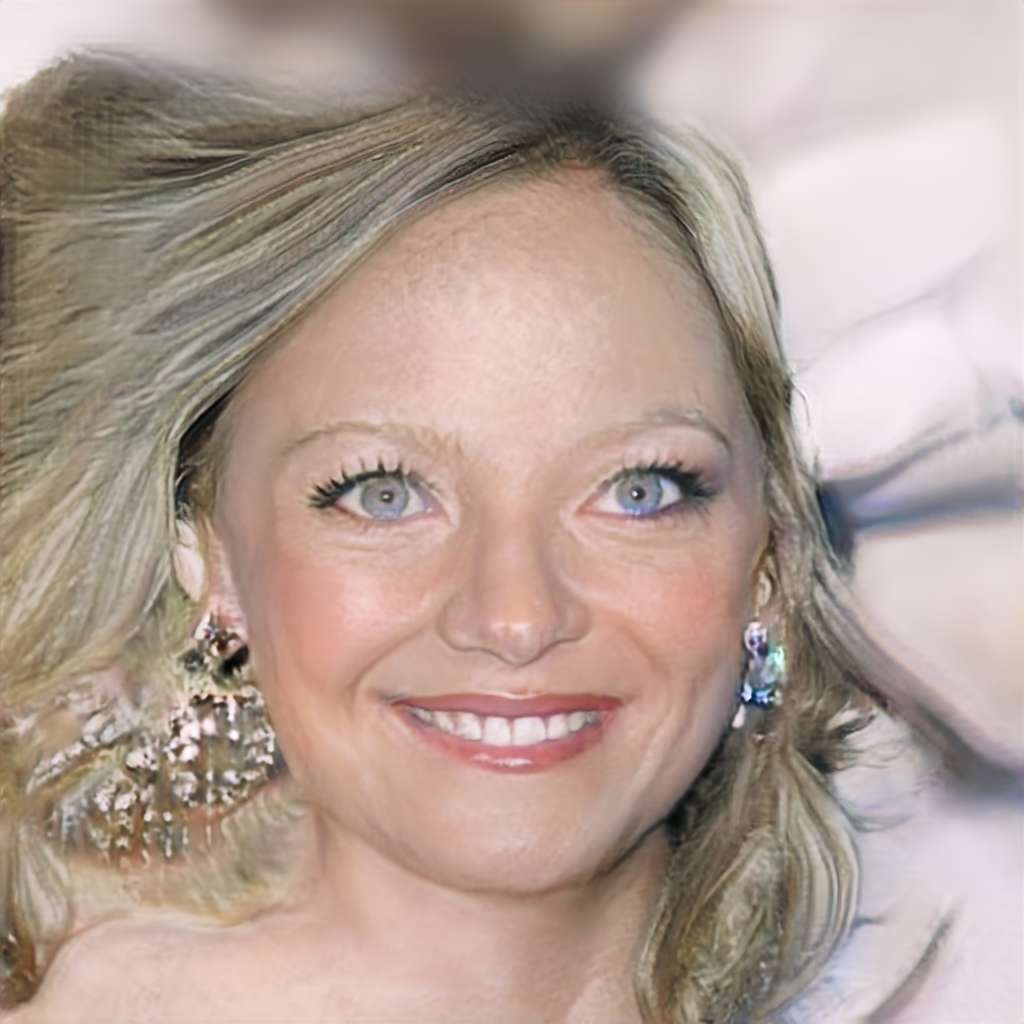
\includegraphics[width=\pganw]{figures/pgan/58_base_iso_reject.jpg}} &
\unreal{
\includegraphics[width=\pganw]{figures/pgan/59_base_iso_reject.jpg}} &
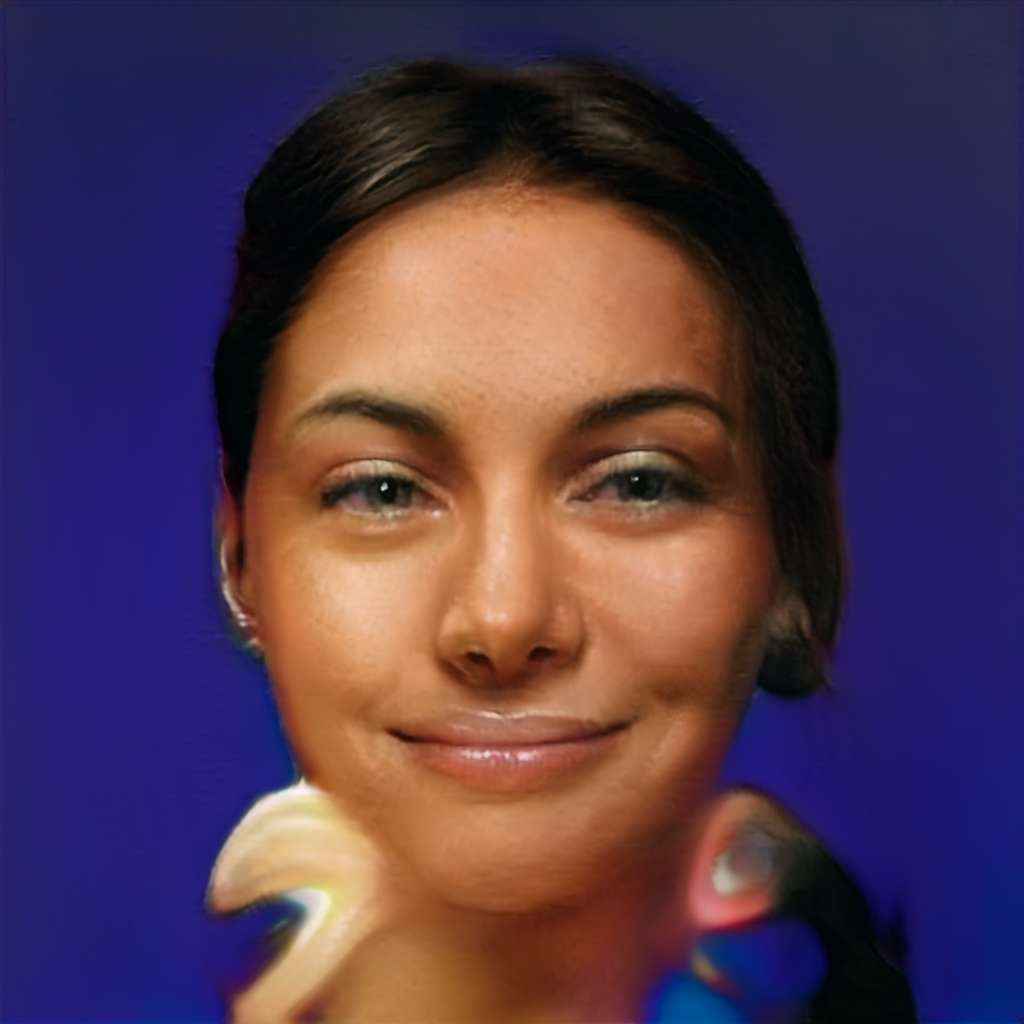
\includegraphics[width=\pganw]{figures/pgan/58_base_iso_MH.jpg} &
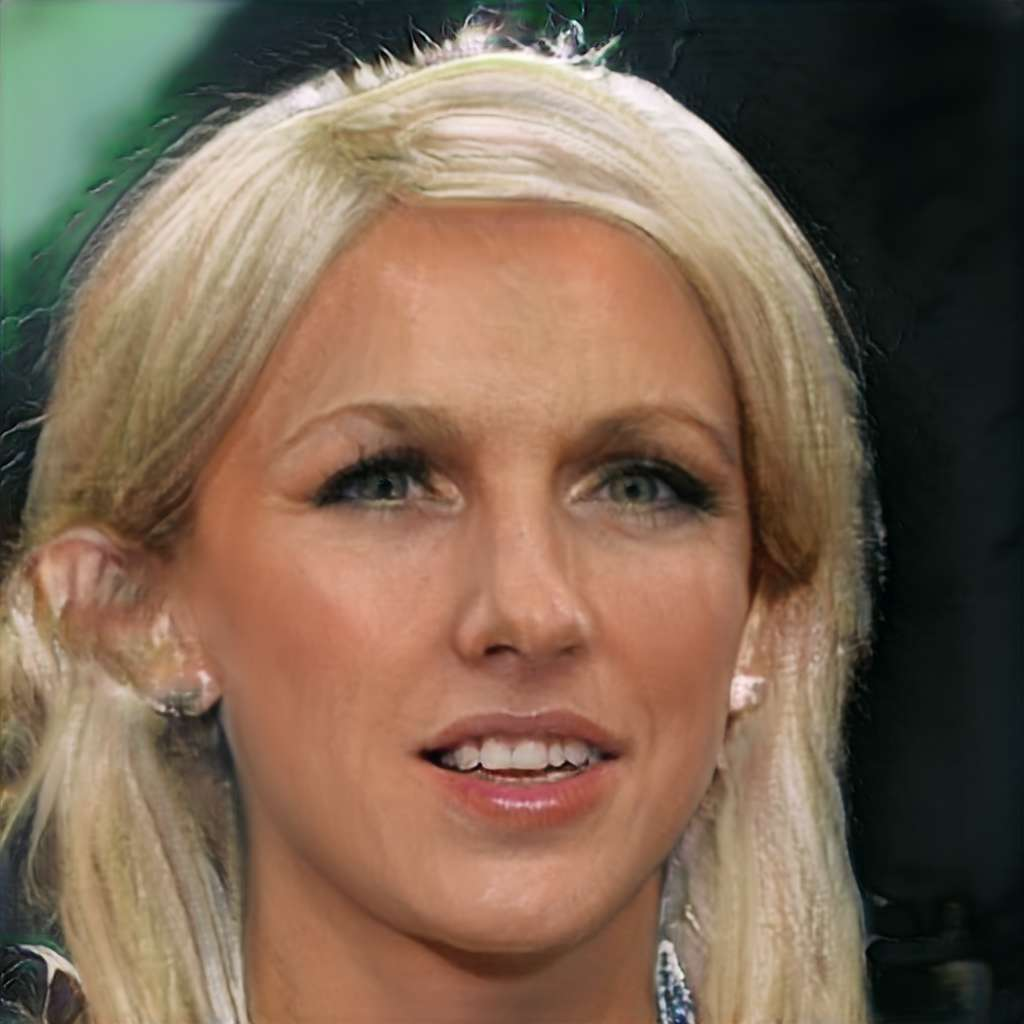
\includegraphics[width=\pganw]{figures/pgan/59_base_iso_MH.jpg} \\
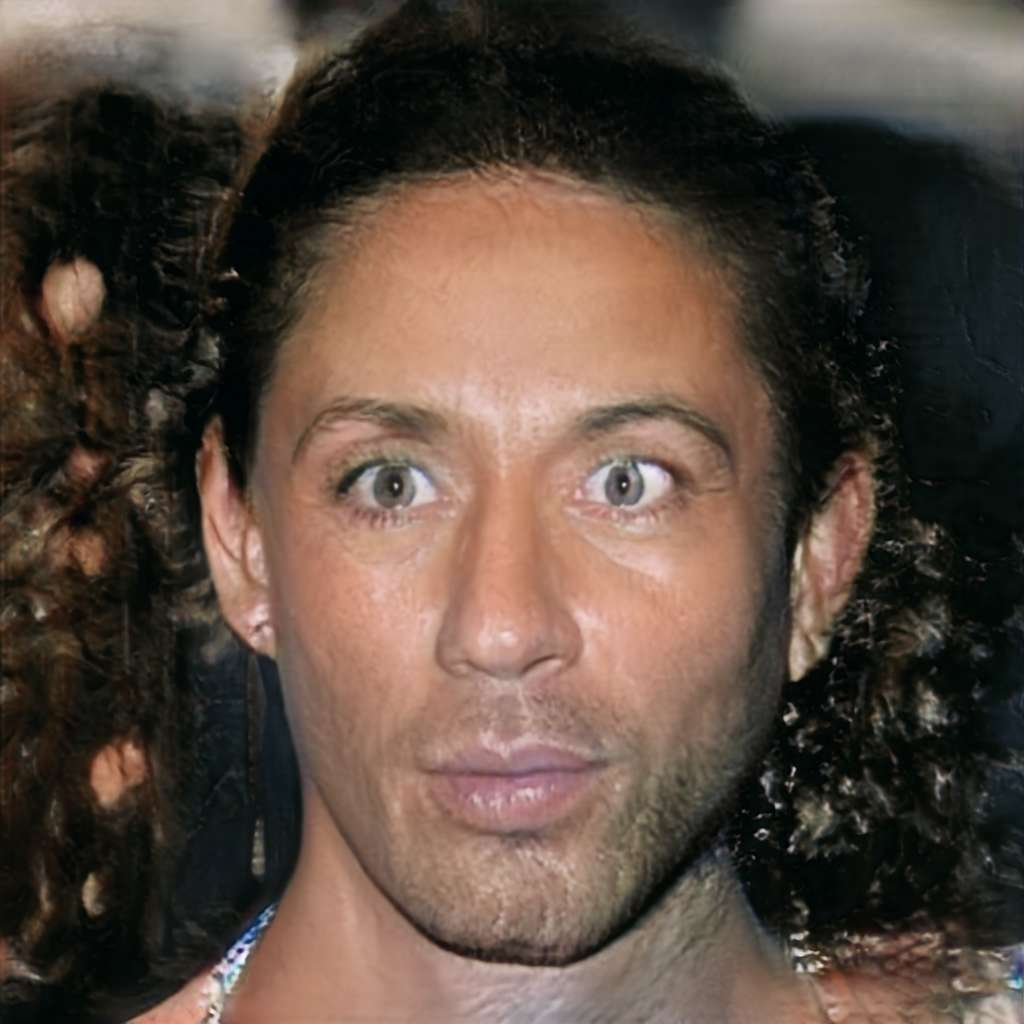
\includegraphics[width=\pganw]{figures/pgan/60_base_iso_base.jpg} &
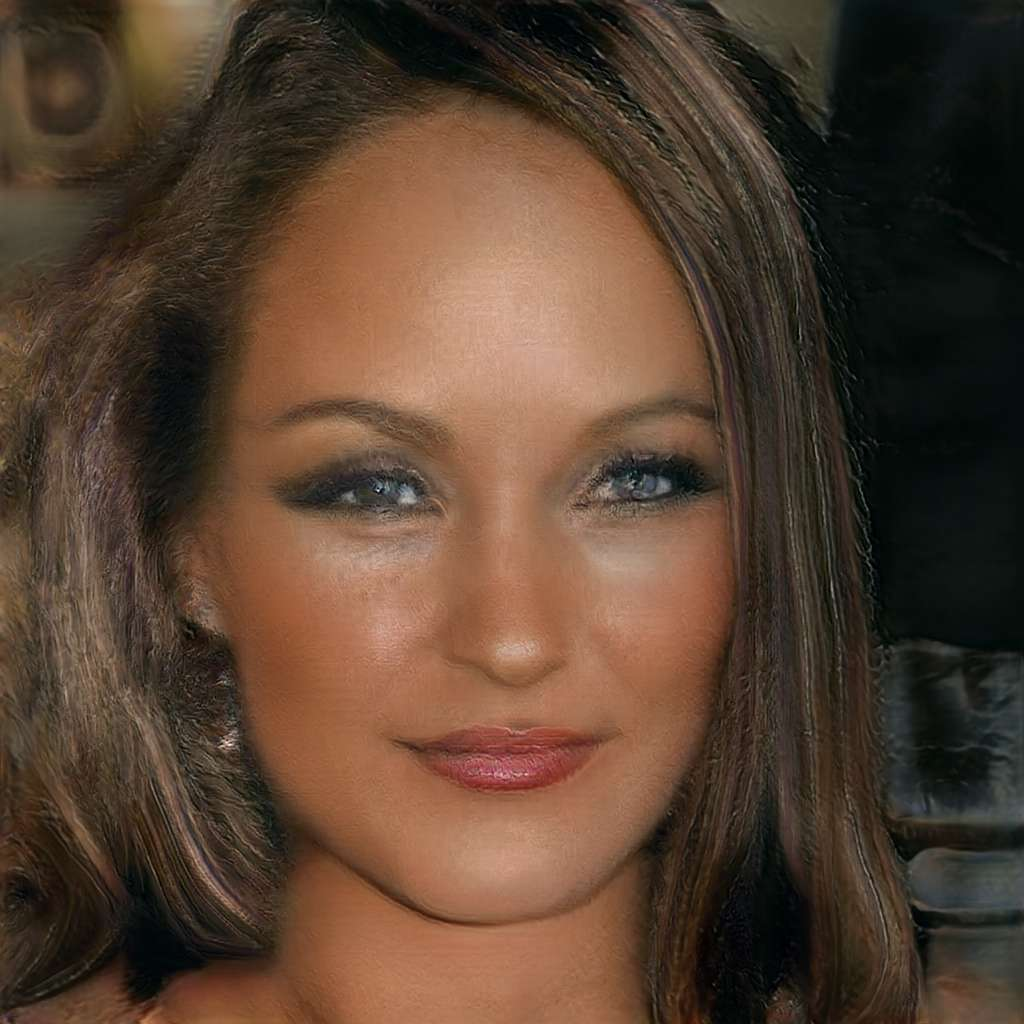
\includegraphics[width=\pganw]{figures/pgan/61_base_iso_base.jpg} &
\includegraphics[width=\pganw]{figures/pgan/60_base_iso_reject.jpg} &
\includegraphics[width=\pganw]{figures/pgan/61_base_iso_reject.jpg} &
\includegraphics[width=\pganw]{figures/pgan/60_base_iso_MH.jpg} &
\includegraphics[width=\pganw]{figures/pgan/61_base_iso_MH.jpg} \\
\unreal{\includegraphics[width=\pganw]{figures/pgan/62_base_iso_base.jpg}} &
\unreal{\includegraphics[width=\pganw]{figures/pgan/63_base_iso_base.jpg}} &
\includegraphics[width=\pganw]{figures/pgan/62_base_iso_reject.jpg} &
\includegraphics[width=\pganw]{figures/pgan/63_base_iso_reject.jpg} &
\includegraphics[width=\pganw]{figures/pgan/62_base_iso_MH.jpg} &
\unreal{\includegraphics[width=\pganw]{figures/pgan/63_base_iso_MH.jpg}} \\
\end{tabular}
\end{center}
\end{table*}

\FloatBarrier

\section*{Acknowledgements}
We thank Rosanne Liu and Zoubin Ghahramani for useful discussions and comments.

\bibliography{mgan_refs}
\bibliographystyle{icml2019}

\end{document}
